%% 
%% Copyright 2019-2024 Elsevier Ltd
%% 
%% This file is part of the 'CAS Bundle'.
%% --------------------------------------
%% 
%% It may be distributed under the conditions of the LaTeX Project Public
%% License, either version 1.3c of this license or (at your option) any
%% later version.  The latest version of this license is in
%%    http://www.latex-project.org/lppl.txt
%% and version 1.3c or later is part of all distributions of LaTeX
%% version 1999/12/01 or later.
%% 
%% The list of all files belonging to the 'CAS Bundle' is
%% given in the file `manifest.txt'.
%% 
%% Template article for cas-sc documentclass for 
%% double column output.

\documentclass[a4paper,fleqn]{cas-sc}

% If the frontmatter runs over more than one page
% Use the longmktitle option.

%\documentclass[a4paper,fleqn,longmktitle]{cas-sc}

%\usepackage[numbers]{natbib}
%\usepackage[authoryear]{natbib}
\usepackage[numbers]{natbib}
%% The amssymb package provides various useful mathematical symbols
\usepackage{amssymb}
%% The amsmath package provides various useful equation environments.
\usepackage{amsmath}
\usepackage{epstopdf}
\usepackage{mathptmx,mathtools}
\usepackage{subcaption}
\usepackage{float} % Add this in your preamble
\usepackage[export]{adjustbox}
\usepackage{array} % Needed for m{} column type


\usepackage{amsmath}
\usepackage{nicefrac}
\usepackage{dirtytalk}
\usepackage{graphicx}   % For including images
\usepackage{tikz}       % For drawing arrows
\usepackage{xcolor}     % For coloring

\newif\ifhighlight   % defines a conditional \ifhighlight

% Turn highlighting ON:
\highlighttrue

% Turn highlighting OFF:
%\highlightfalse

% Define the highlight macro:
\ifhighlight
\newcommand{\hl}[1]{\textcolor{blue}{#1}} % or \textcolor{red}{#1}
\else
\newcommand{\hl}[1]{#1} % does nothing, just prints the text
\fi

\usepackage{lineno}
\renewcommand\linenumberfont{\normalfont\bfseries\small} % <-- Increase line number size

%%%Author macros
\def\tsc#1{\csdef{#1}{\textsc{\lowercase{#1}}\xspace}}
\tsc{WGM}
\tsc{QE}
%%%

% Uncomment and use as needed
%\newtheorem{theorem}{Theorem}
%\newtheorem{lemma}[theorem]{Lemma}
%\newdefinition{rmk}{Remark}
%\newproof{pf}{Proof}
%\newproof{pot}{Proof of Theorem \ref{thm}}

\begin{document}
	
	
	\let\WriteBookmarks\relax
	\def\floatpagepagefraction{1}
	\def\textpagefraction{.001}
	
	% Short title
	\shorttitle{Data-Driven Analysis of Rising Bubbles}    
	
	% Short author
	\shortauthors{B.K. Majd et al.}  
	
	% Main title of the paper
	\title[mode=title]{On Data-Driven Methods for Buoyancy-Driven Rising Bubble within Eulerian, Lagrangian, and \hl{Moving-Eulerian} Frameworks}  
	
	
	% Authors (all with the same affiliation)
	\author[1]{Behnam Kazemi Majd}[orcid=0009-0009-2076-4749]  % Add ORCID if available
	\cormark[1]
	\ead{behnam.k.majd@ntnu.no}
	
	\author[1]{Arturo A. Arosemena}
	\author[1]{Sanjid S. Chirammel}
	\author[1]{Jannike Solsvik}
	
	% Affiliation
	\affiliation[1]{organization={Department of Chemical Engineering, Norwegian University of Science and Technology (NTNU)},
		city={Trondheim},
		postcode={N-7491},
		country={Norway}}
	% Corresponding author text
	\cortext[cor1]{Corresponding author}

	
	
	
	\begin{abstract}
		The present study extends and compares the applicability of two data-driven methods—Proper Orthogonal Decomposition (POD) and Dynamic Mode Decomposition (DMD)—for estimating the rise characteristics of a buoyancy-driven bubble deforming across rectilinear, transitional, and oscillatory regimes. Training datasets are obtained from two previously validated in-house multiphase solvers: the  Interface Level Set Method on a co-located grid (SI-LSM$_{\text{col}}$) and the Conservative Diffuse Interface (CDI) method. The study evaluates the accuracy of reconstructed bubble interface, rise velocity, and trajectory based on reduced-order models derived from POD and DMD, applied within Eulerian, Lagrangian, and \hl{moving-Eulerian} frameworks. The accuracy is quantified using the Frobenius norm of relative field-reconstruction errors. Results show that frameworks can be ranked in descending order of accuracy as Lagrangian, \hl{moving-Eulerian}, and Eulerian. While the Lagrangian framework yields the lowest reconstruction error of 0.19 ± 0.10 \%, it suffers from particle-to-grid interpolation artifacts, leading to inaccurate rise velocity and false indications of bubble breakage. In contrast, the \hl{moving-Eulerian} approach offers a field-reconstruction error of 1.6 ± 1.4 \%, along with a noise-free approximation of the bubble interface and rise velocity. The efficiency of data-driven methods decreases for 3D bubbles with greater deformation, requiring more modes to maintain reconstruction accuracy. POD consistently outperforms DMD as it requires fewer modes across all frameworks. Notably, DMD struggles to reconstruct the bubble interface during early rise stages, while POD remains robust throughout. Finally, inaccuracies in the interface affect the rise velocity value, as locating the bubble interface precedes velocity sampling.
		
	\end{abstract}
	
	% Research highlights
	\begin{highlights}
		\item Compares data-driven methods for state estimation of rising bubbles in different frames
		\item Finds POD generally outperforms DMD for accurate, low-order reconstructions.
		\item \hl{Moving-Eulerian} approach balances accuracy with manageable cost.
		\item Lagrangian frame offers best precision but suffers from interpolation noise.
		\item Provides guidance for reduced-order modeling of complex multiphase flows.
	\end{highlights}
	
	
	% Keywords
	% Each keyword is separated by \sep
	\begin{keywords}
		3D rising bubble \sep data-driven methods \sep POD \sep DMD \sep Lagrangian framework
	\end{keywords}
	
	\maketitle
	
	\linenumbers
	
	%% Use \section commands to start a section
	\section{Introduction}
	\label{Introduction}
	
	The problem of a single rising bubble has a wide range of contemporary applications across different industries, including heat~\cite{Larimi2018} and mass transfer~\cite{Kentheswaran2023}, optimized use of antibiotics~\cite{Hamdollahi2022}, ship stability~\cite{Fang2022}, and acoustic radiation~\cite{Ouyang2021}. Since the 1950s, researchers have studied the dynamics of a rising bubble, particularly characteristic parameters such as rise velocity and path instability~\cite{Saffman1956,TSUGE1977,Duineveld1995}, and this continues to the present day~\cite{Shi2024,Bonnefis2024,Hosen2024}. Furthermore, recent experimental and numerical studies have shown that these characteristic parameters--path instability, rise velocity, and also deformation--of a raising bubble are affected by a plethora of effects \cite{Liu2006,Cano-Lozano2016,Kure2021}, making it challenging to propose predictive models that remain accurate across different flow regimes and fluid properties. In this context, the applicability, assessment, and subsequent advancement of existing models purely based on data are considered key for improving predictions about rising bubble behavior.
	
	Data-driven decomposition techniques, commonly known as reduced-order models (ROMs), extract the dominant spatial and temporal patterns—referred to as \textit{modes}, a type of coherent structure—from either experimental or numerical simulations. In fact, they are categorized as a group of post-processing tools that capture the essential flow physics, without resolving the governing equations and solely based on available data. \citet{Lumley1967166} was the first to employ a data-driven method, the proper orthogonal decomposition (POD)~\cite{volkwein2013proper,Berkooz1993}, for extracting coherent structures. \citet{Holmes1996} extended the method to provide a low-dimensional representation of turbulent flows. \citet{SCHMID2010} developed the dynamic mode decomposition (DMD) algorithm that could provide valuable insights into the underlying dynamics of the system, such as growth and decay rates of the structures extracted from the flow fields. Various research groups later extended these classical data-driven methods (consider, e.g., the spectral POD~\cite{Towne2018}, higher-order DMD~\cite{LeClainche2017}, multi-scale POD~\cite{Mendez2019}, and multi-resolution DMD~\cite{Kutzz2016a}) with the purpose of overcoming their limitations in particular applications. For example, spectral POD can capture structures with low energy or at multiple frequencies, while multi-scale POD can be applied to flow fields with multiple temporal or spatial scales. Similarly, the traditional data driven methods may require further improvements to address their shortcomings when applied to convection dominated problems. In this case, \citet{Lu2020} showed that a simply change of framework may be enough. Their findings suggest that data-driven techniques are more efficient in the Lagrangian framework in convection-diffusion problems. \hl{In the context of a rising bubble, these techniques can provide a low-order representation of complex bubble dynamics—such as wake instabilities—through an in-depth analysis of the extracted modes. Depending on the flow regime and the level of complexity, the number of modes required to represent the full dynamics can vary substantially, and selecting an appropriate decomposition method that yields the fewest possible modes remains a persisting challenge.} In this convection-dominated flow problem, the translational dynamics are intricate to analyze, and the bubble may experience severe interface deformation and various flow regimes, further increasing the complexity that makes the traditional data-driven methods inefficient. Recent studies have made a great effort to analyze the efficiency of the interface reconstruction of a 2D bubble. \citet{Yin2023a} investigated the efficiency of DMD and Lagrangian DMD in reconstructing the bubble interface with a rectilinear rising path. Their findings suggest that Lagrangian DMD performs more efficiently. Additionally, they demonstrated that incorporating a velocity-prediction procedure is essential for accurately reconstructing deforming bubbles, highlighting the limitations of classical data-driven methods. An extension of their work is the development of a bubble-tracking DMD method~\cite{Yin2023} in which experimental datasets of a rising bubble in the oscillatory region were used. 
	
	Although recent studies have suggested using DMD to analyze a 2D rising bubble from a Lagrangian perspective, key questions and challenges remain unexplored, requiring further investigation. One critical question is whether data-driven techniques are robust across different rising stages, including rectilinear, transition, and oscillatory. Additionally, the efficiency of other data-driven techniques, such as POD, has not been systematically compared to DMD. A crucial challenge is the precision of the Lagrangian approach and its efficiency in estimating the rise velocity of a bubble in 3D scenarios. This will be addressed by applying a \hl{moving-Eulerian} framework as an alternative approach. Finally, this work aims to examine the effectiveness of data-driven methods in calculating rising characteristics such as rise velocity and trajectory, as the previous works mainly focused on the bubble interface. 
	
	In summary, the outlined challenges and questions have inspired us to investigate the application of data-driven techniques, including POD and DMD, in analyzing a rising bubble as a ROMs for state estimation. By pursuing this direction, the current work sets out to compare the efficacy of POD and DMD to estimate critical rise characteristics, such as terminal velocity, rise trajectory, and the bubble interface during the entire rising process, including the rectilinear, transition, and the oscillatory stages at different frames of reference simulated in two different coordinate systems\textemdash two-dimensional \textit{axisymmetric} and three-dimensional \textit{Cartesian} coordinate systems. The outcome of the work provides a comprehensive evaluation of the considered data-driven approaches for bubble dynamics and identifies their limitations as reduced-order tools within different frameworks. \hl{The findings of this paper can be used as a roadmap for mode analysis by identifying an efficient decomposition method that uses a small number of modes.}
	
	The work is organized as follows. Section~\ref{Mathematical formulation} presents the numerical methodologies used to obtain the datasets for the analysis. The three different working frameworks are briefly introduced in section~\ref{Framework}. Section~\ref {Data-driven methods} discusses the theoretical formulation of data-driven methods. Section~\ref{Results and discussion} investigates the efficiency of different methods for five cases of a rising bubble within the different frameworks, followed by conclusions in section~\ref{Conclusion}.
	
	
	\section{Mathematical formulation}
	\label{Mathematical formulation}
	In this section, a brief discussion on mathematical formulations and numerical methodologies utilized by two in-house Computational multi-Fluid Dynamics solvers\textemdash Sharp Interface Level Set Method on Co-located grid (SI-LSM$_{\text{col}}$) \cite{Chirammel2023} and Conservative Diffuse Interface (CDI)~\cite{Jain2020}\textemdash for obtaining the flow fields required by the data-driven techniques is presented.  The Direct Numerical Simulation (DNS) datasets are obtained from the solution of conservation equations using SI-LSM$_{\text{col}}$ on an \textit{axisymmetric} coordinate system and CDI on a 3D \textit{Cartesian} coordinate system. The choice of SI-LSM$_{\text{col}}$ and CDI on different coordinate systems is purposely made: the former is computationally less expensive for Lagrangian tracking, while the latter can produce bubbles with oscillatory rising paths. Furthermore, the present CDI method and SI-LSM$_{\text{col}}$ utilize a \textit{whole-domain conservation law}-based formulation and a \textit{sub-domain conservation law}-based formulation with interfacial jump boundary condition, respectively. Validation of these in-house solvers and detailed discussion on the numerical methodology are presented elsewhere \cite{Chirammel2023, Salimi2025}, whereas for clarity, the utilized non-dimensional conservation equations are given here as follows
	\subsection*{Continuity Equation:}
	\begin{equation}\label{eqt:continuity}
		\nabla\cdot\mathbf{U}=0
	\end{equation}
	\subsection*{Momentum equation:}
	\noindent For SI-LSM$_{\text{col}}$:
	\begin{equation}\label{eqt:momEqt-SI}
		\frac{\partial(\chi_{i}\mathbf{U})}{\partial\tau}+\nabla\cdot(\chi_{i}\mathbf{U}\mathbf{U})=-\nabla P+\frac{1}{Re}\nabla\cdot(\eta_{i}[\nabla\mathbf{U}+\nabla\mathbf{U}^T])-\frac{\chi_{i}}{Fr^2}\hat{j}
	\end{equation}
	\noindent For CDI:
	\begin{equation}\label{eqt:UnifiedMomentumEquation-Conservation}
		\frac{\partial(\rho^{*}\mathbf{U})}{\partial\tau}+\nabla\cdot((\rho^*\mathbf{U}-(1-\chi)\mathbf{R})\mathbf{U})=-\nabla P+\frac{1}{Re}\nabla\cdot(\mu^{*}[\nabla\mathbf{U}+\nabla\mathbf{U}^T])-\frac{\rho^*}{Fr^2}\hat{j}+\frac{\kappa}{We}\nabla \phi_{CDI}
	\end{equation}
	where $\tau$, $\mathbf{U}$, $P$, $\kappa$, and $\hat{j}$ are the non-dimensional time, velocity vector, pressure, interface curvature, and unit vector along the Y-axis in the 3D \textit{Cartesian} and Z-axis in the \textit{axisymmetric} coordinate systems, respectively. Whereas, the regularization term R is given as
	
	\begin{equation*}
		R = \Upsilon \bigg[\epsilon\nabla\phi_{CDI}-\phi_{CDI}(1-\phi_{CDI})\frac{\nabla\phi_{CDI}}{|\nabla\phi_{CDI}|}\bigg]
	\end{equation*}
	
	\noindent where $\Upsilon$ is the regularization parameter. Utilizing the bubble diameter as the length scale $D$, the gravitation acceleration $g$, velocity scale $u_c=\sqrt{gD}$, and time scale $t_c=D/u_c$, various non-dimensional variables are given as
	\begin{equation*}
		\mathbf{X}=\frac{\mathbf{x}}{D}; \mathbf{U}=\frac{\mathbf{u}}{u_c}; \tau=\frac{t}{t_c}; P=\frac{p}{\rho_1u_c^2}
	\end{equation*}
	and the corresponding non-dimensional governing parameters are
	\begin{equation*}
		We=\frac{\rho_1 u_c^2D}{\sigma}; \ Bo=\frac{\rho_1gD^2}{\sigma}; \ Re=\frac{\rho_1Du_c}{\mu_1}; \ Fr=\frac{u_c}{\sqrt{gD}}
	\end{equation*}
	where $We$, $Bo$ , $Re$, and $Fr$ are the Weber number (inertia-to-surface tension ratio), Bond number (buoyancy-to-surface tension ratio), Reynolds number (inertia-to-viscous force ratio) and Froude (inertia-to-gravity ratio), respectively. Here, $\rho$, $\mu$, and $\sigma$ are the density, dynamic viscosity, and surface tension, respectively. 
	
	\begin{figure}[!htbp]
		\centering
		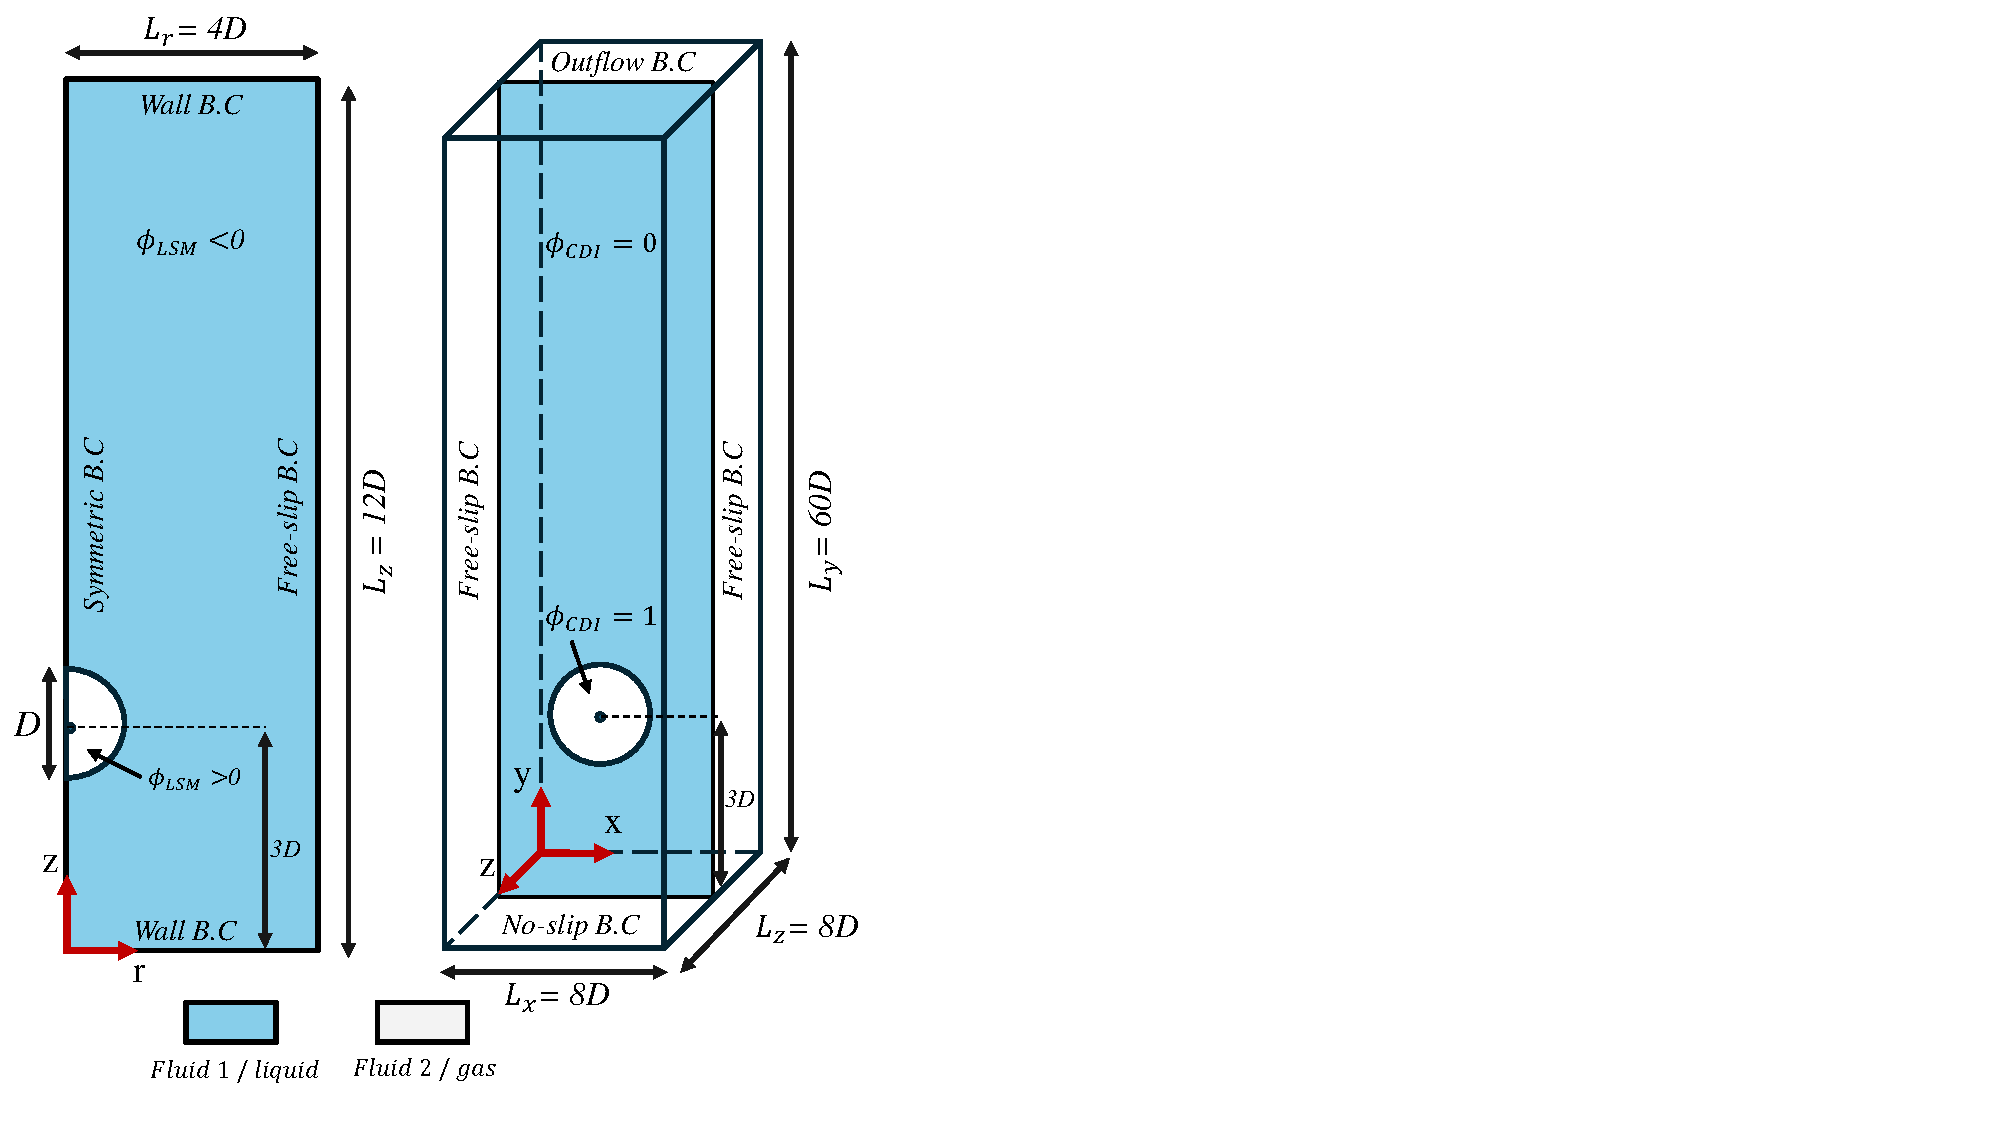
\includegraphics[scale=0.5,trim={0.1cm 0.5cm 18cm 0cm},clip]{Figure1.pdf}
		\put(-125,250){\textbf{(b)}}
		\put(-225,250){\textbf{(a)}}
		\caption{Schematic of the computational domain for rising bubble simulation on a) two-dimensional \textit{axisymmetric} with SI-LSM$_{\text{col}}$ and b) three-dimensional \textit{Cartesian} configuration with CDI.}
		\label{Fig1}
	\end{figure}
	
	Further, the non-dimensional physical properties of the fluids are defined as
	\newline
	\noindent For SI-LSM$_{\text{col}}$:  
	\begin{equation*}
		\begin{aligned}
			&\chi_{i}=H(\phi_{LSM}) + \chi H(\phi_{LSM})\\
			&\eta_{i}=H(\phi_{LSM}) + \eta H(\phi_{LSM})
		\end{aligned}
	\end{equation*}
	where
	\begin{equation*}
		\chi=\frac{\rho_2}{\rho_1}\text{ and }\eta=\frac{\mu_2}{\mu_1}
	\end{equation*}
	and
	\begin{equation}\label{eqt:heaviside_SI}
		H(\phi_{LSM})=\begin{cases}
			1&\phi_{LSM}\ge0\\
			0&\phi_{LSM}< 0
		\end{cases}
	\end{equation}
	\newline
	\noindent For CDI:
	\begin{equation*}
		\begin{aligned}
			&\rho^{*}=\phi_{CDI} + \chi \phi_{CDI}\\
			&\mu^{*}=\phi_{CDI} + \eta \phi_{CDI}
		\end{aligned}
	\end{equation*}
	where $\phi_{LSM}$ and $\phi_{CDI}$ are the level-set and phase-field functions, respectively. The level-set function represents two fluids with positive and negative values, and the $\phi_{LSM}=0$ contour corresponds to the interface separating the two fluids. The phase-field function utilizes the values 0 and 1 to represent the fluids and interface with $\phi_{CDI}=0.5$ contour.
	
	For the present SI, the momentum equation is solved along with an interfacial jump boundary condition, given as 
	\begin{equation}\label{eqt:Pressure_JumpBC}
		[P]= P_{1,\Gamma}-P_{2,\Gamma}=\frac{\kappa}{We}+\frac{2}{Re}(\eta_{1}-\eta_{2})\hat{N}\cdot(\nabla U\cdot\hat{N},\nabla V\cdot\hat{N})
	\end{equation}
	where the subscripts 1, 2, and $\Gamma$ correspond to fluid-1, fluid-2 and interface, respectively. Further, $\hat{N}$ is the unit normal and defined as 
	
	\begin{equation}\label{eqt:heaviside_SI}
		\hat{N}=\begin{cases}
			\frac{\nabla\phi_{LSM}}{|\nabla\phi_{LSM}|} & for~~SI$-$LSM_{col}\\ \\
			\frac{\nabla\phi_{CDI}}{|\nabla\phi_{CDI}|} & for~~CDI
		\end{cases}
	\end{equation}
	
	\subsubsection*{Interface Advection Equation:}
	\noindent For SI-LSM$_{\text{col}}$:
	\begin{equation}\label{eqt:LSadvection}
		\frac{\partial\phi_{LSM}}{\partial\tau}+\mathbf{U}\cdot\nabla\phi_{LSM}=0
	\end{equation}
	\noindent For CDI:
	\begin{equation}\label{eqt:CDIadvectioneqt}
		\frac{\partial\phi_{CDI}}{\partial\tau}+\nabla\cdot(\mathbf{U}\phi_{CDI})=\nabla\cdot\Upsilon\bigg[\epsilon\nabla\phi_{CDI}-\phi_{CDI}(1-\phi_{CDI})\frac{\nabla\phi_{CDI}}{|\nabla\phi_{CDI}|}\bigg]
	\end{equation} 
	where $\epsilon$ is the regularization parameters with values $\mathbf{U}_{max}$ and $\Delta X$ utilized in this study, respectively. 
	
	Further for SI, the advected $\phi_{LSM}$ is reinitialized as a normal distance function by solving a reinitialization equation, given as
	\begin{equation}\label{eqt:reinitialization}
		\frac{\partial\phi_{LSM}}{\partial\tau_s}=S_{\epsilon}(\phi_{LSM,0})(1-|\nabla\phi_{LSM}|)
	\end{equation}
	where $\tau_s$ and $S_{\epsilon}$ denotes pseudo time step and smoothened sign function \cite{Sussman1994}, defined as
	\begin{equation*}
		\tau_s=\frac{\Delta X}{10} \text{ and } S_{\epsilon}=\sqrt{\frac{\phi_{LSM,0}}{\phi_{LSM,0}^2+\Delta X^2}}
	\end{equation*} 
	
	\noindent where $\phi_{LSM,0}$ corresponds to the $\phi_{LSM}$ value before pseudo iteration in Eq. (9)
	
	%%%%%%%%%%%%%%%%%%%%%%%%%%%%%%%%%%%%%%%%%%%%%%%%%%%%%%
	%%%%%%%%%%%%%%%%%%%%%%%%%%%%%%%%%%%%%%%%%%%%%%%%%%%%%%
	%%%%%%%%%%%%%%%% Table 1 %%%%%%%%%%%%%%%%%%%%%%%%%
	%%%%%%%%%%%%%%%%%%%%%%%%%%%%%%%%%%%%%%%%%%%%%
	\begin{table}[!htbp]
		\begin{center}
			\caption{Non-dimensional physical properties of the fluids utilized for simulating various cases along with obtained terminal shape and number of snapshots. All cases are simulated on a grid size of $D/40$, along with a constant density and viscosity ratio of 10. Note, $Fr=1$ and $We=Bo$ for all cases.}
			\vspace{0cm}
			\begin{tabular}{|>{\centering\arraybackslash}m{1.2cm}|c|c|c|m{2.4cm}|c|}
				\hline\hline
				Case & Re & Bo &$D~(m)$&Terminal shape&No. of snapshots\\
				%\\
				%\\
				\hline
				C$_1$ & 20 & 20 & $ 0.30$ & $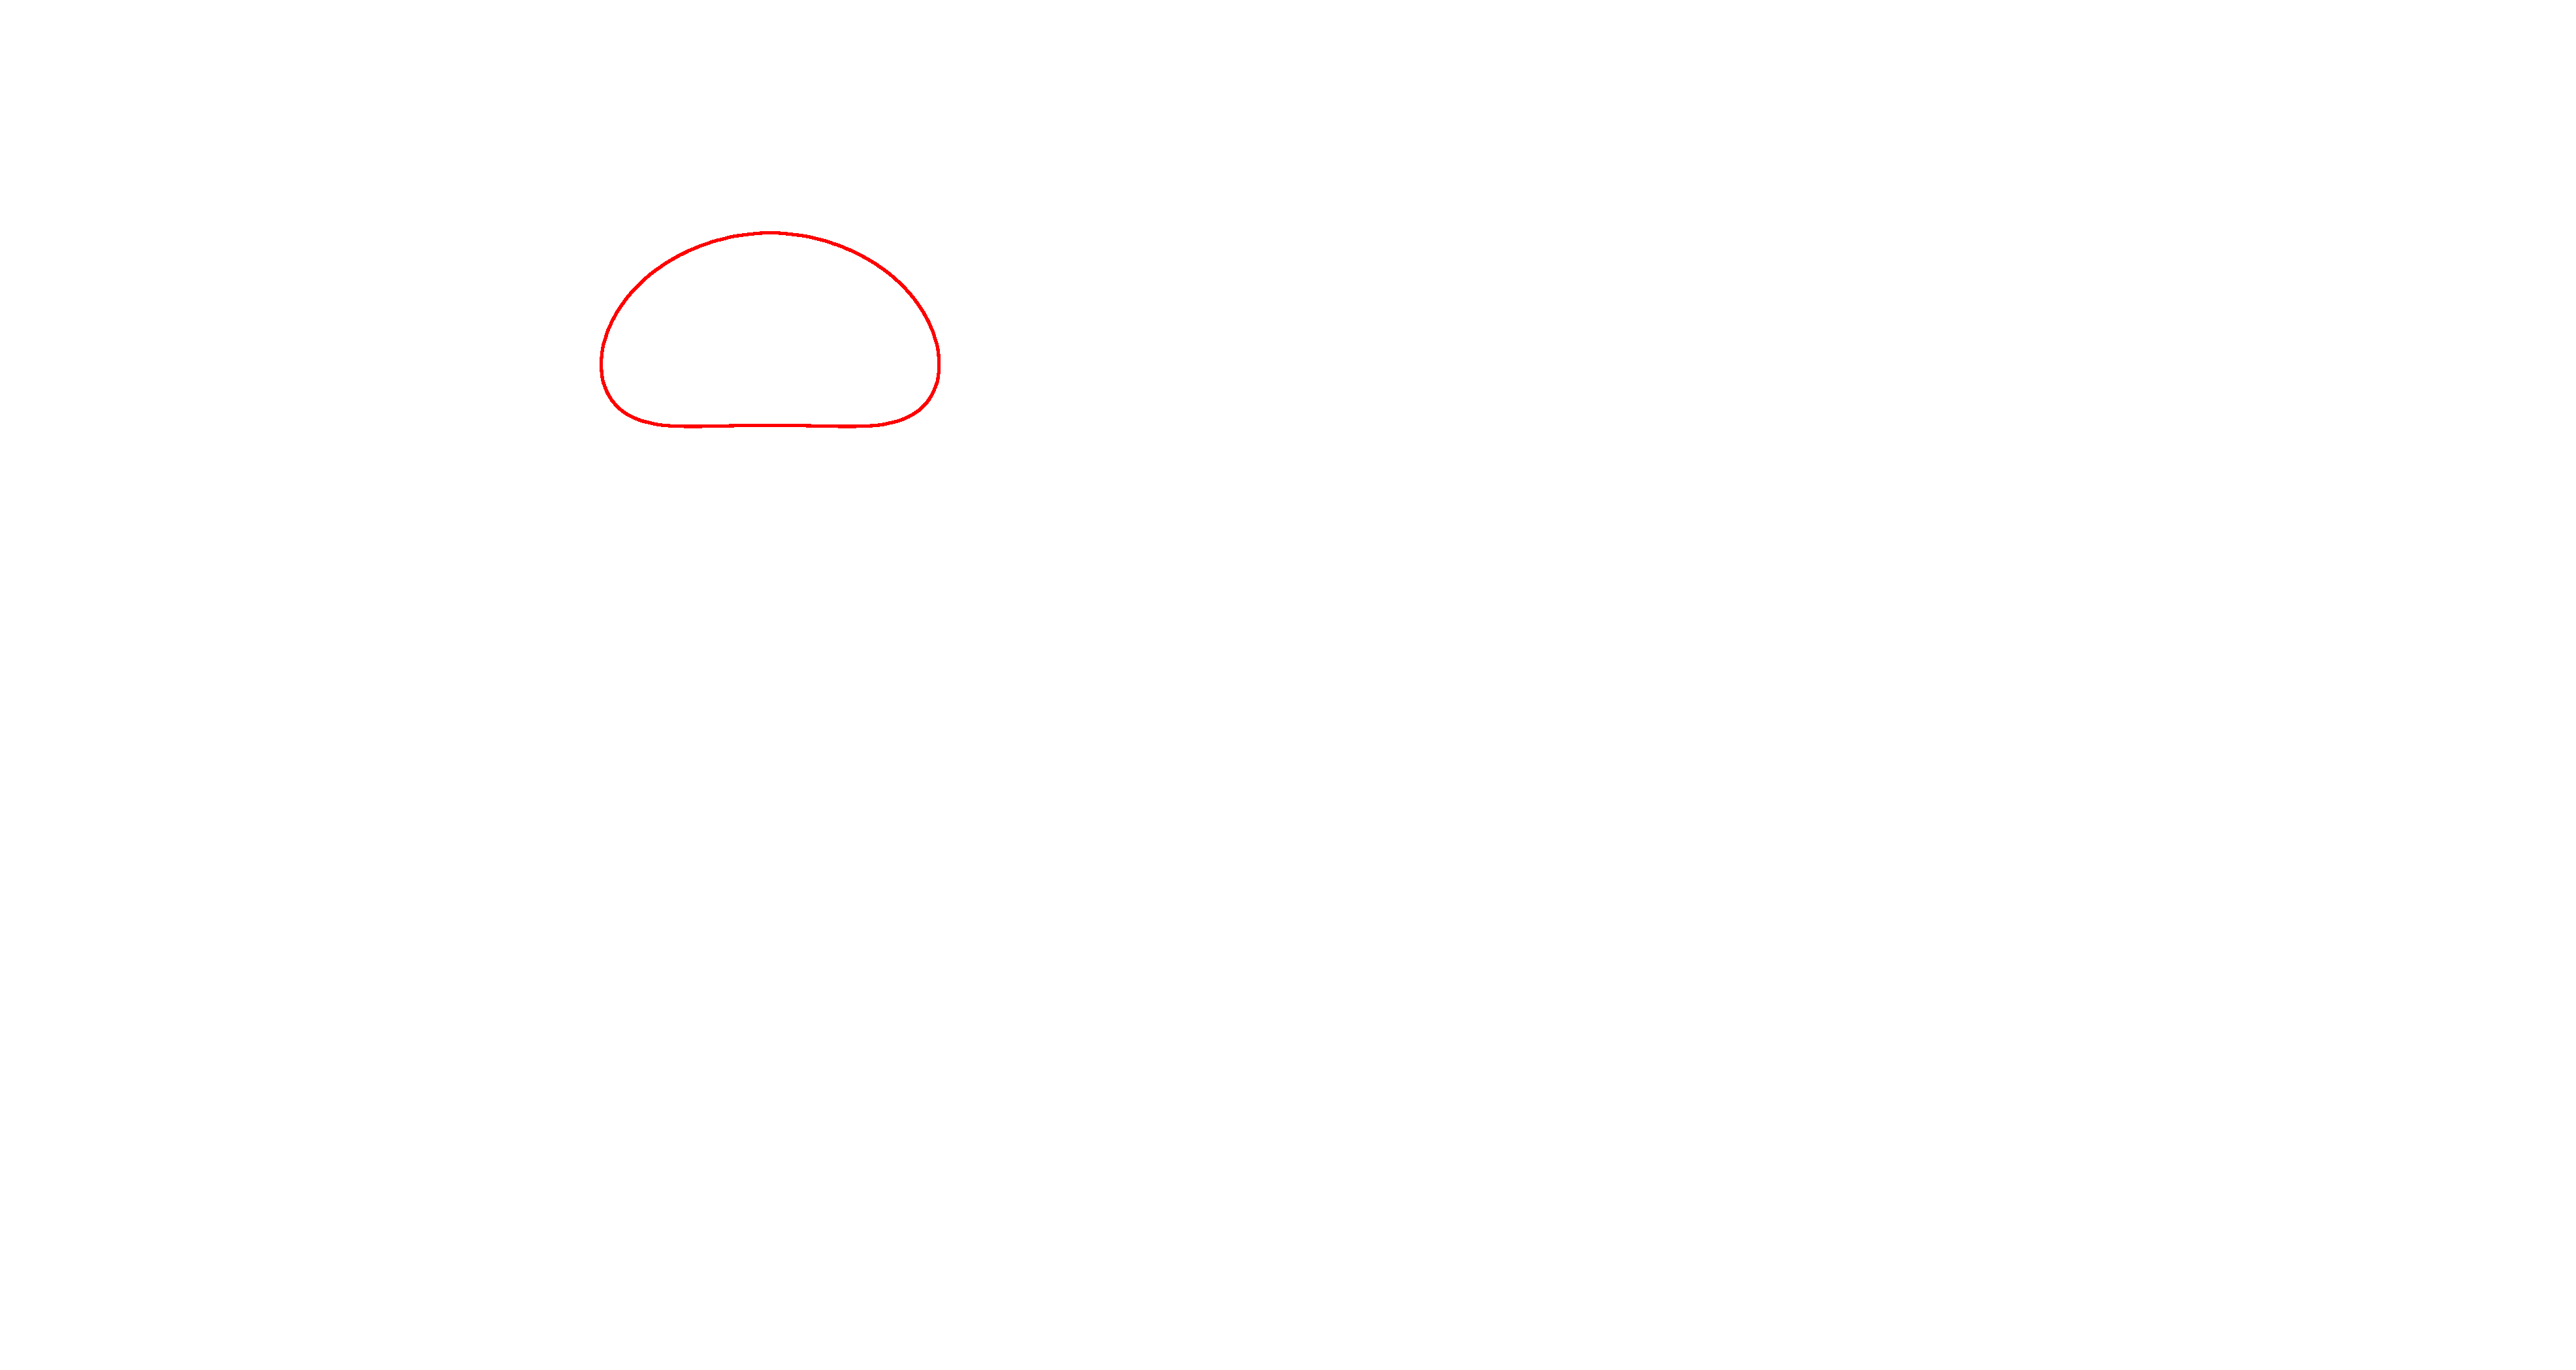
\includegraphics[scale=0.13,trim={10.5cm 23cm 25cm 5cm},clip]{C1.eps}$& 400			%%%%%%%%%%%%%%%%%%%%%%%%%%%%%%%%%%%%%%%%%%%
				%%%%%%%%%%%%%%%%%%%%%%%%%%%%%%%%%%%%%%%%%%%
				%%%%%%%%%%%%%%%%%%%%%%%%%%%%%%%%%%%%%%%
				\\
				\hline
				C$_2$ & 40 & 40 & $ 0.40$ & $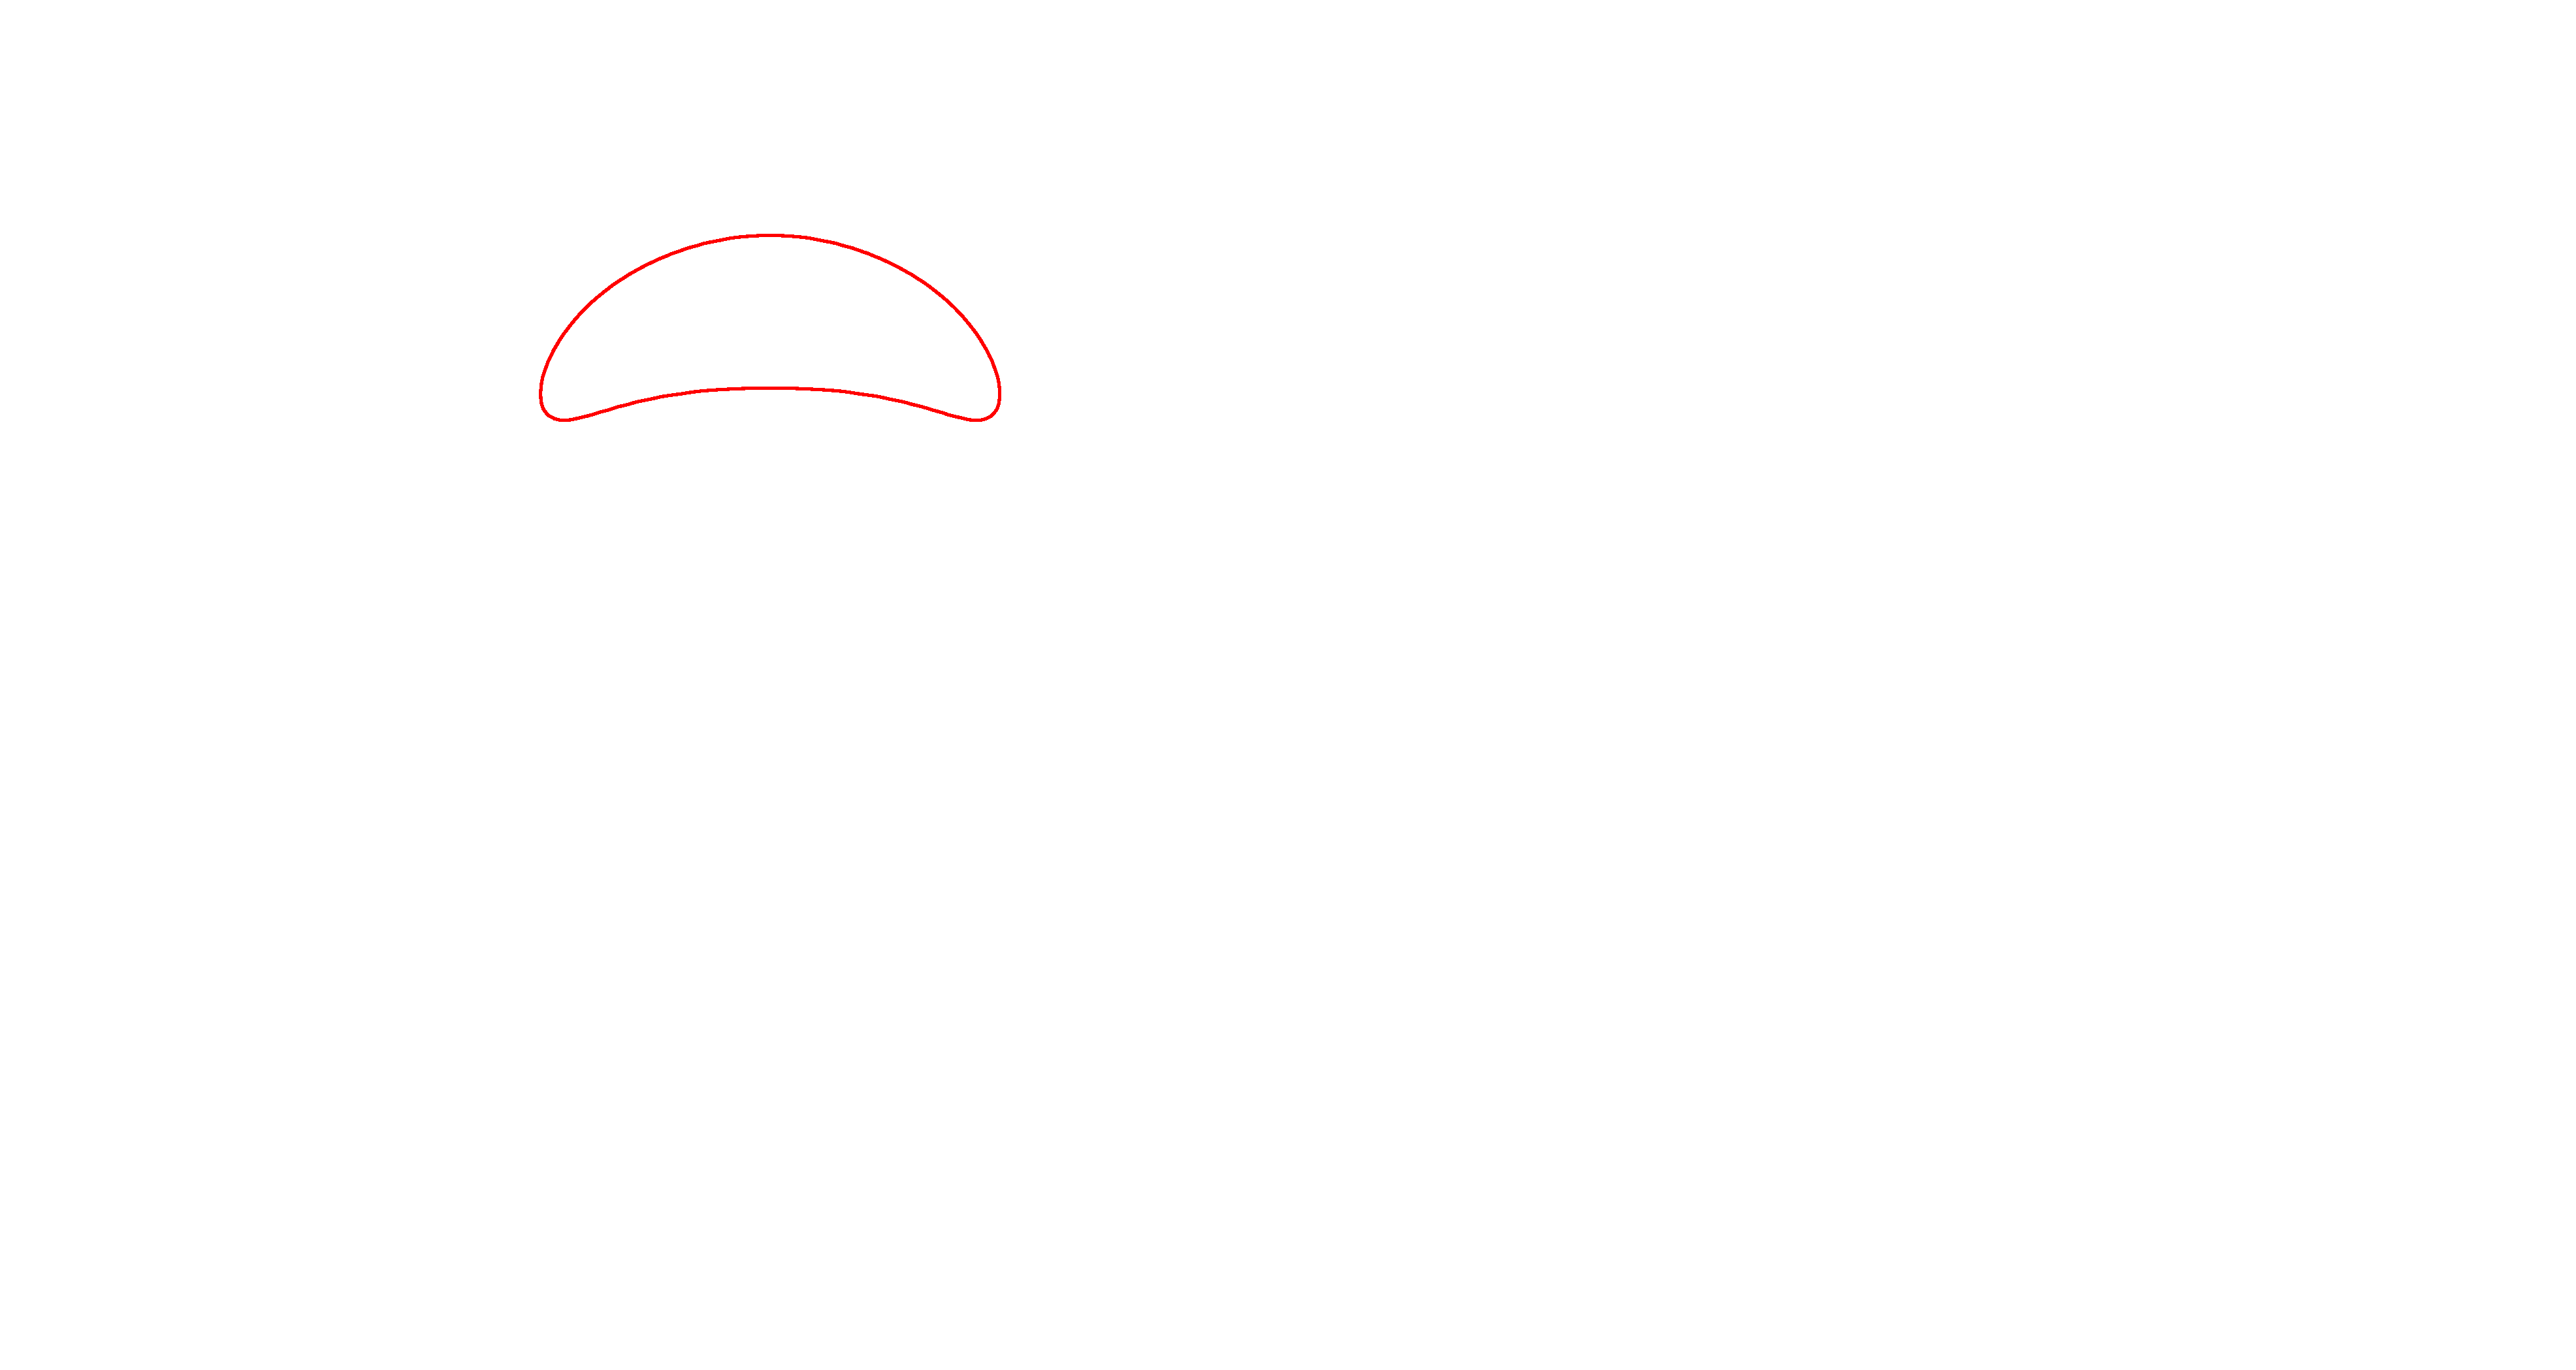
\includegraphics[scale=0.1,trim={8cm 23cm 25cm 5cm},clip]{C2.eps}$& 400
				%%%%%%%%%%%%%%%%%%%%%%%%%%%%%%%%%%%%%%%%%%%
				%%%%%%%%%%%%%%%%%%%%%%%%%%%%%%%%%%%%%%%%%%%
				%%%%%%%%%%%%%%%%%%%%%%%%%%%%%%%%%%%%%%%
				\\
				\hline
				C$_3$ & 100 & 100 & $ 0.63$ & $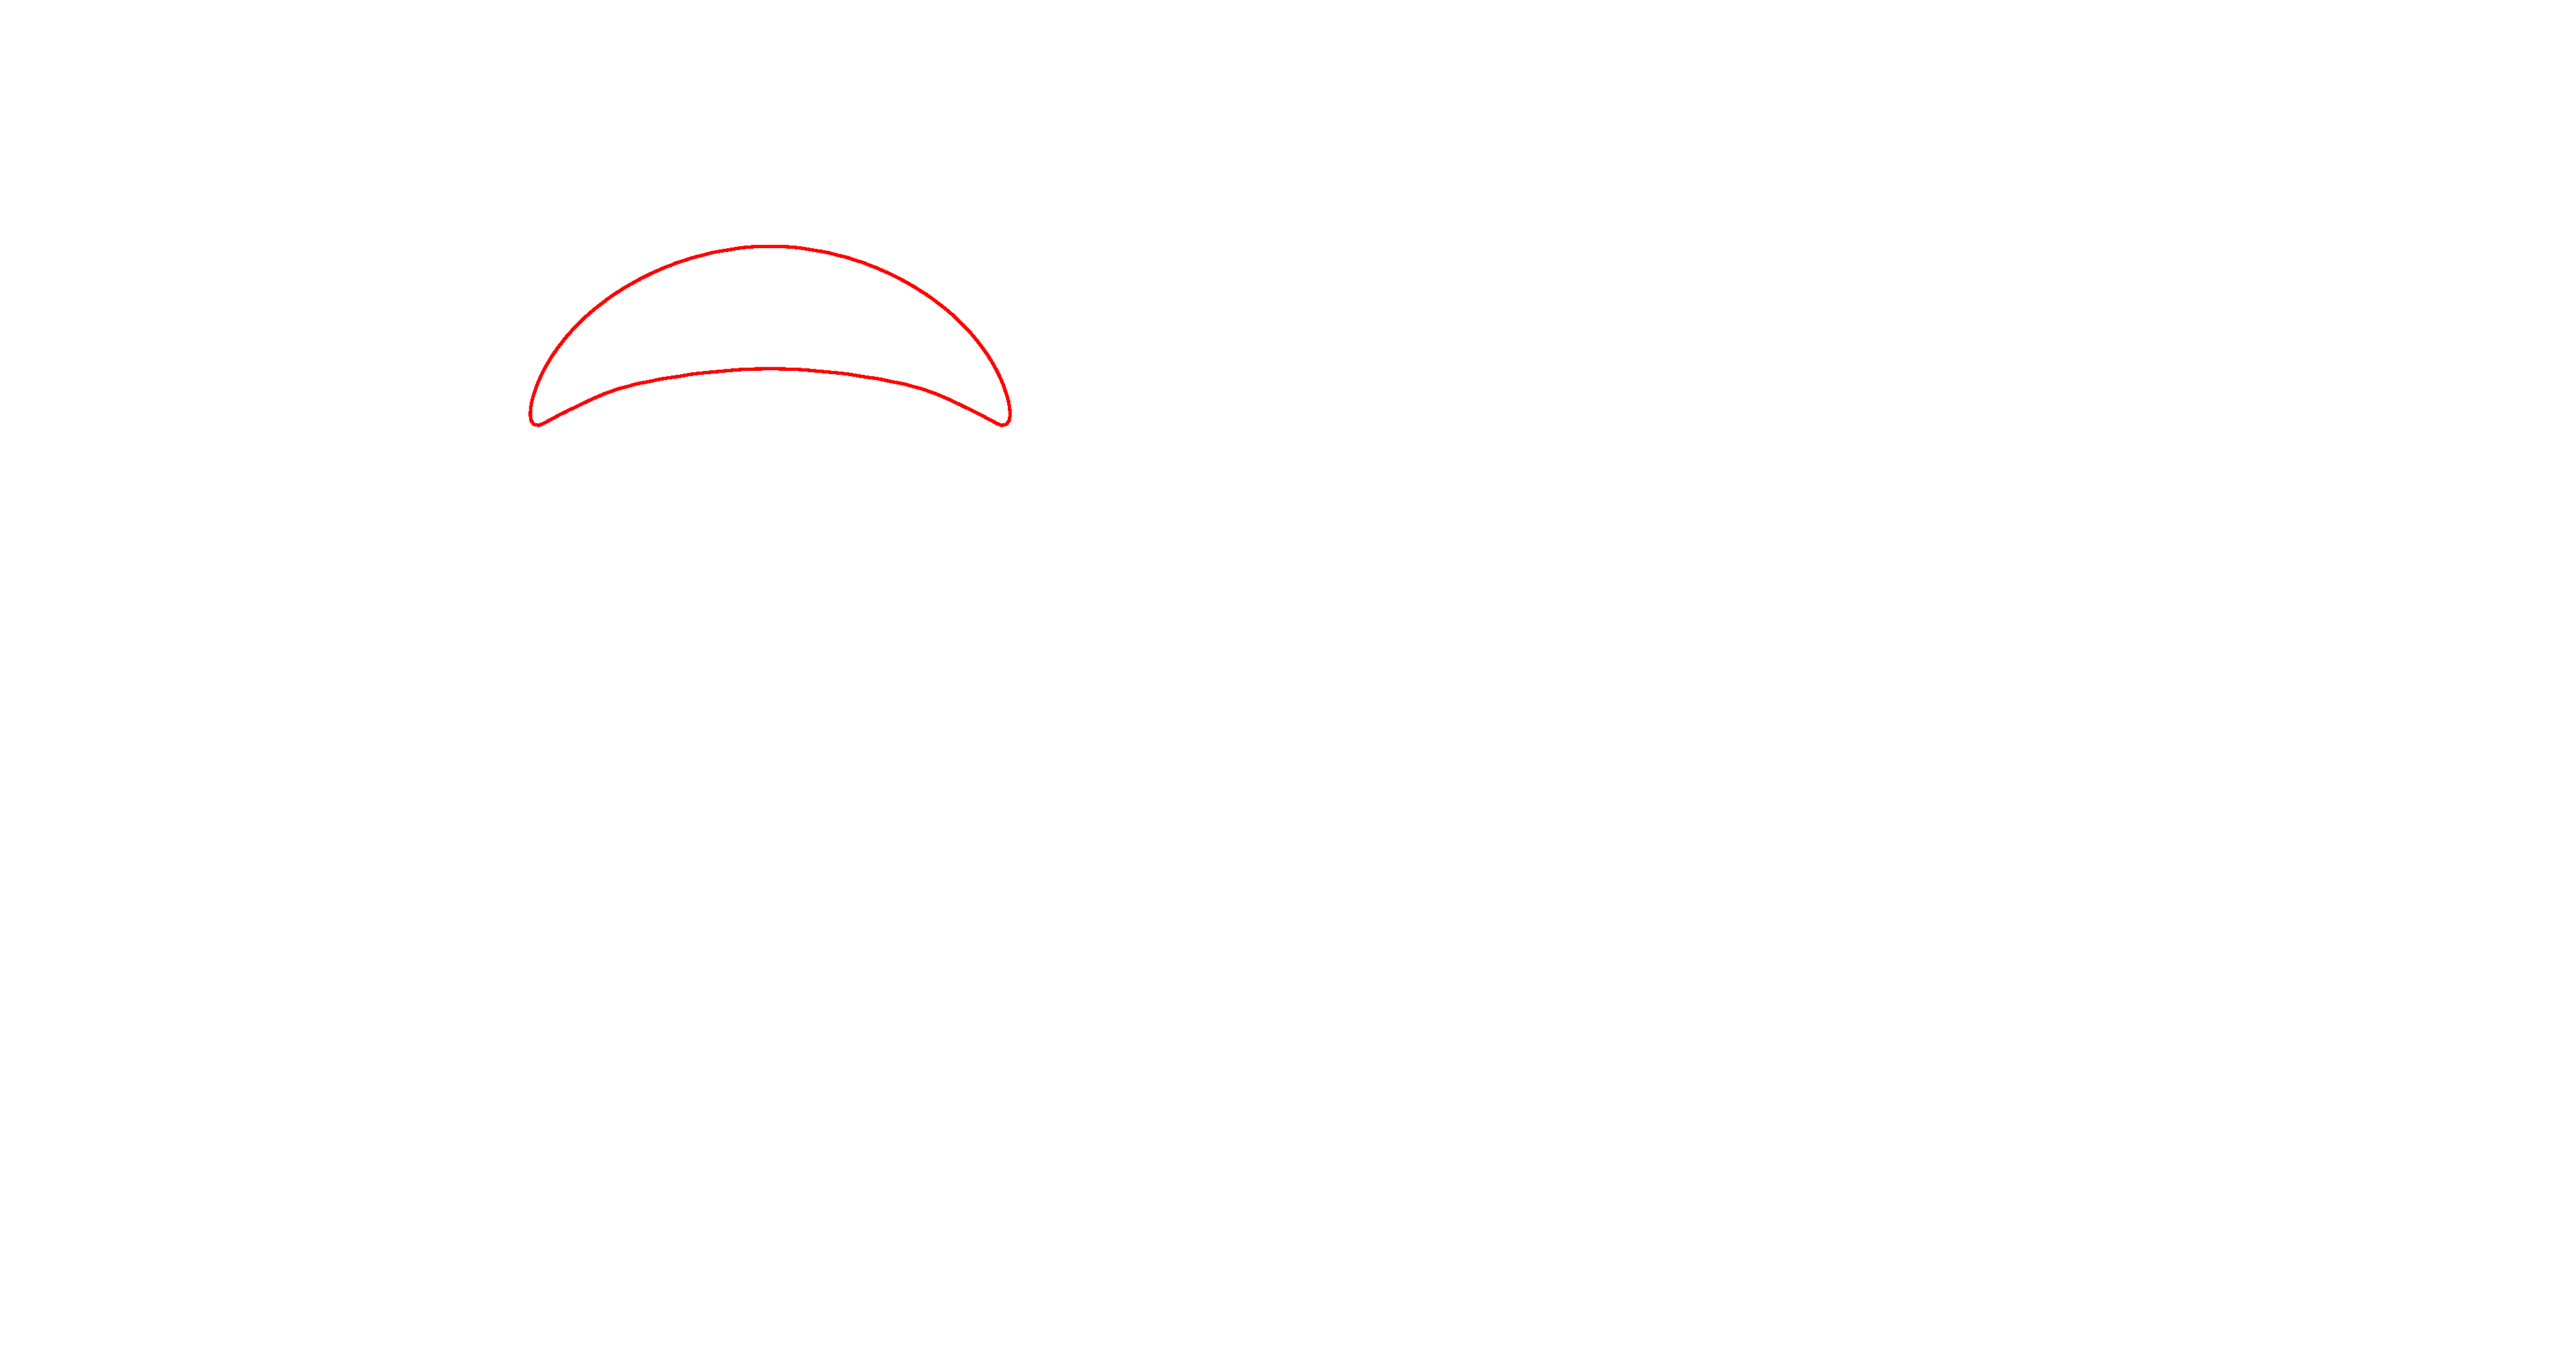
\includegraphics[scale=0.1,trim={8cm 23cm 25cm 5cm},clip]{C3.eps}$& 400
				\\
				%%%%%%%%%%%%%%%%%%%%%%%%%%%%%%%%%%%%%%%%%%%
				%%%%%%%%%%%%%%%%%%%%%%%%%%%%%%%%%%%%%%%%%%%
				%%%%%%%%%%%%%%%%%%%%%%%%%%%%%%%%%%%%%%%
				\hline
				C$_4$ & 168.5 & 2.2 & $ 0.027$& $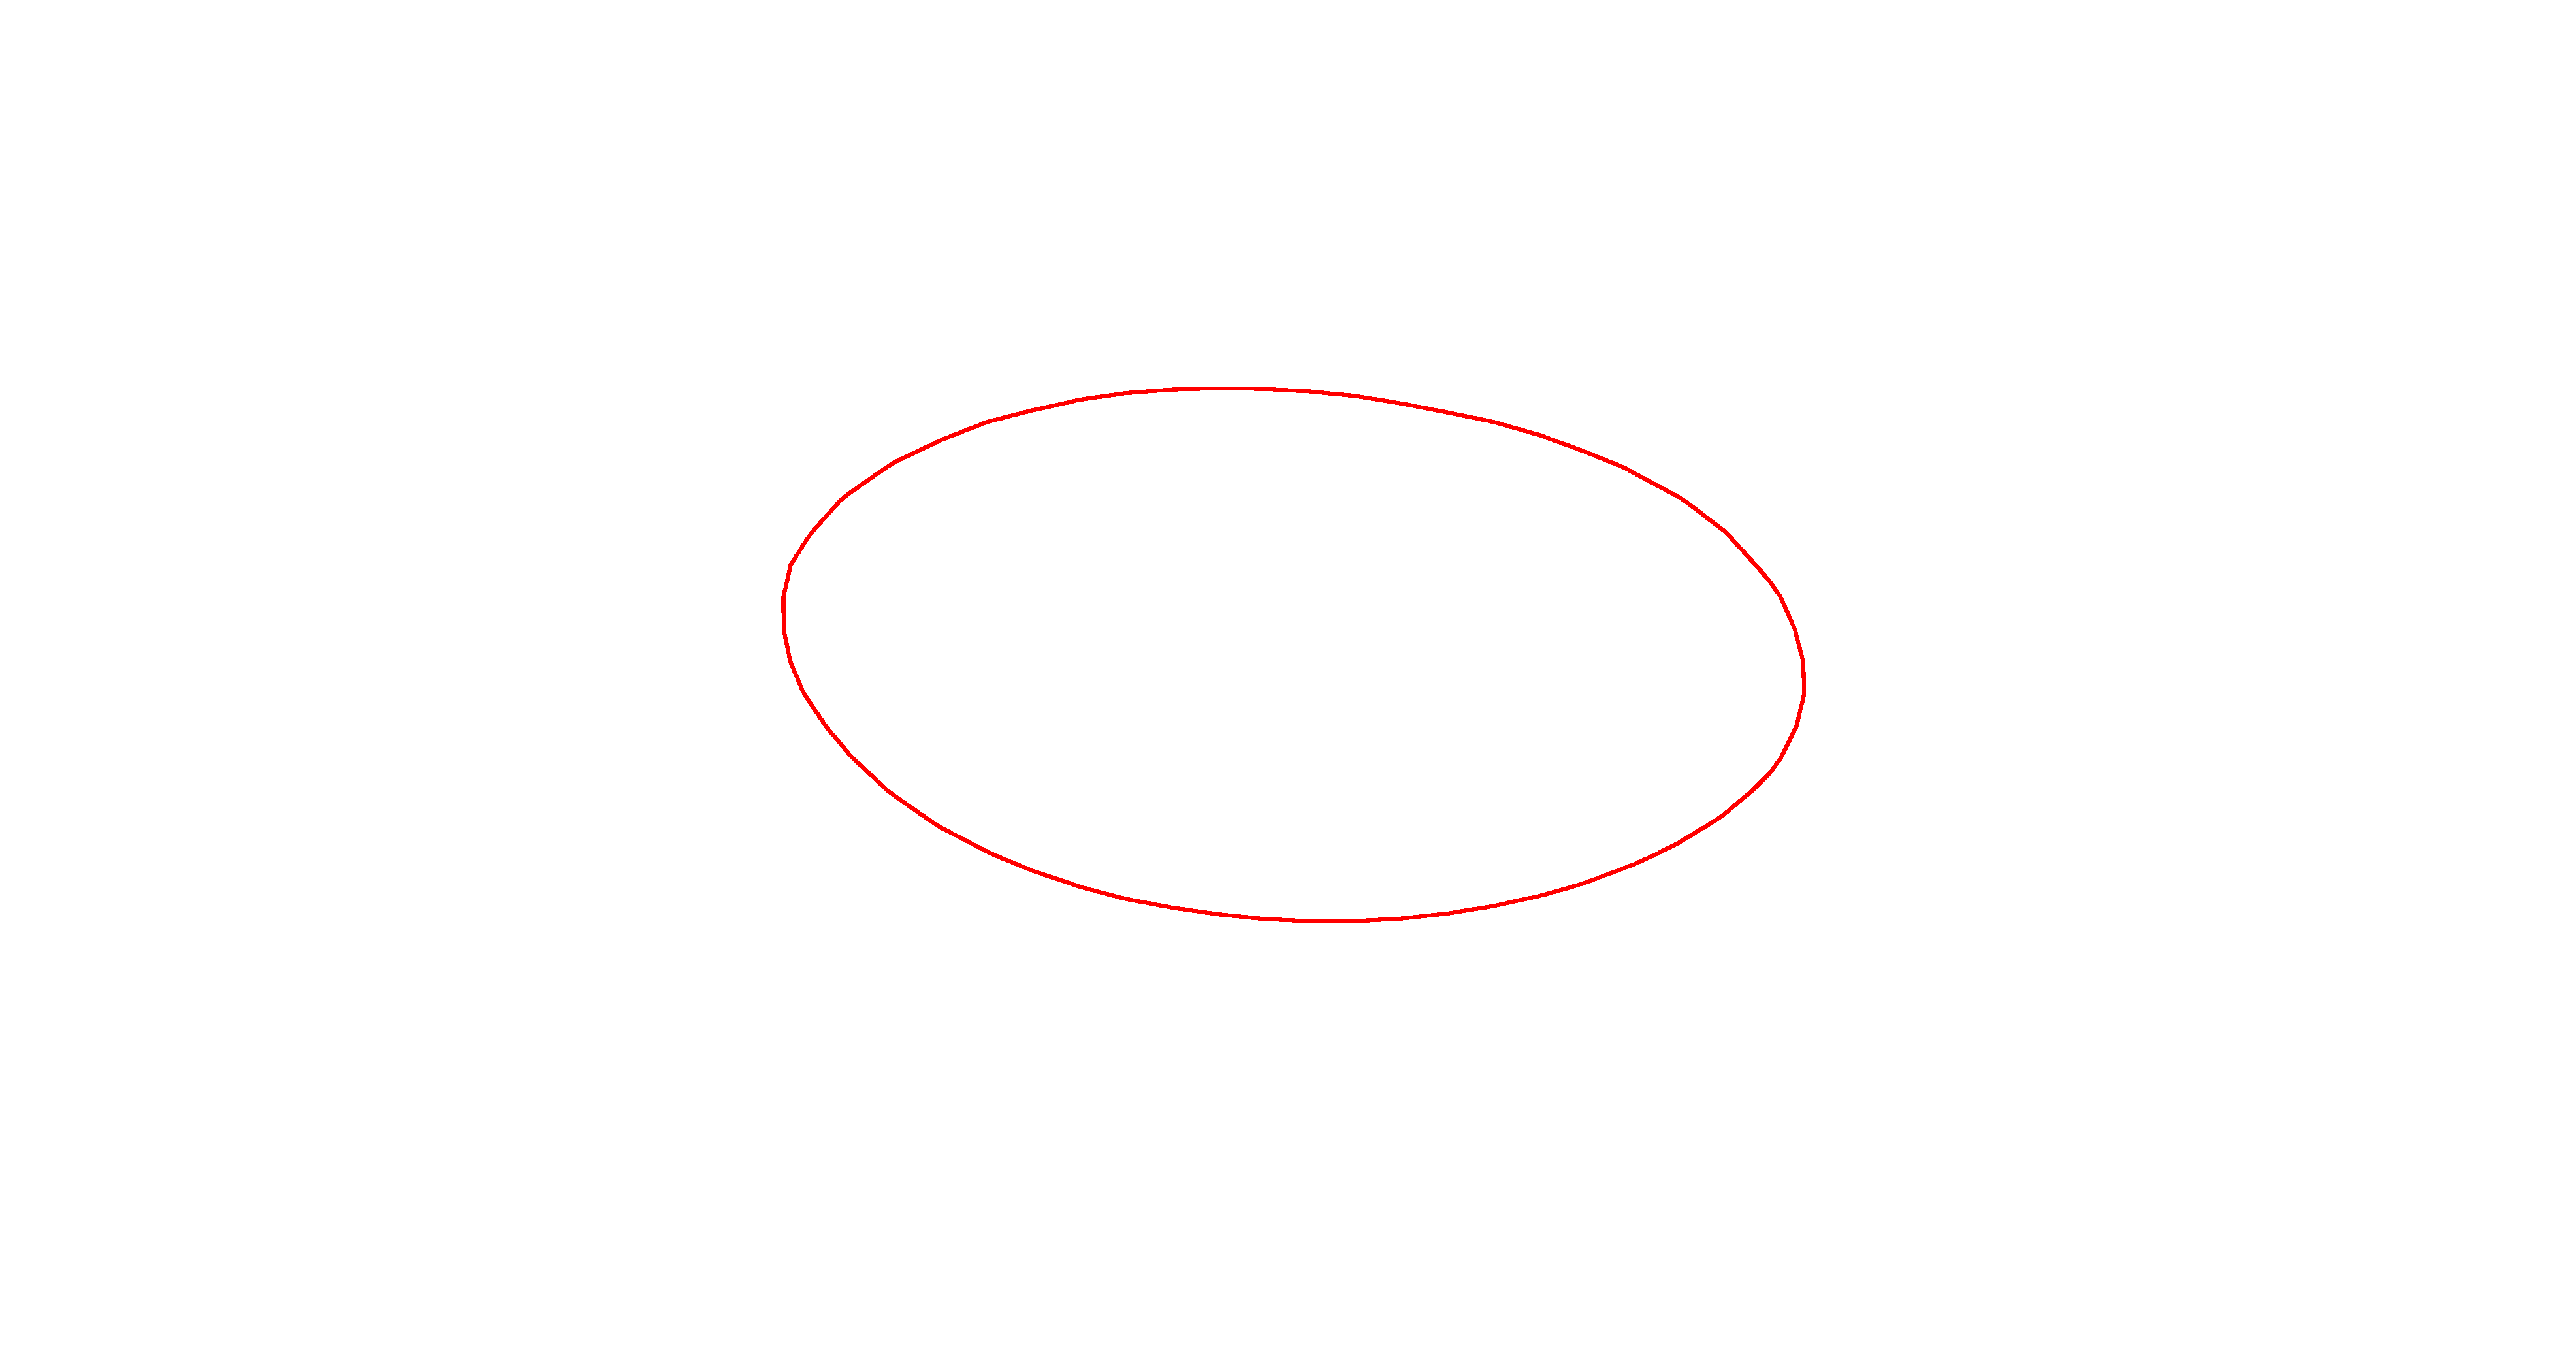
\includegraphics[scale=0.05,trim={10cm 10cm 8cm 8cm},clip]{C4.eps}$& 490
				%%%%%%%%%%%%%%%%%%%%%%%%%%%%%%%%%%%%%%%%%%%
				\\
				%%%%%%%%%%%%%%%%%%%%%%%%%%%%%%%%%%%%%%%%%%%
				%%%%%%%%%%%%%%%%%%%%%%%%%%%%%%%%%%%%%%%%%%%
				%%%%%%%%%%%%%%%%%%%%%%%%%%%%%%%%%%%%%%%
				%\\
				\hline
				C$_5$ & 168.5 & 12 & $ 0.027$& $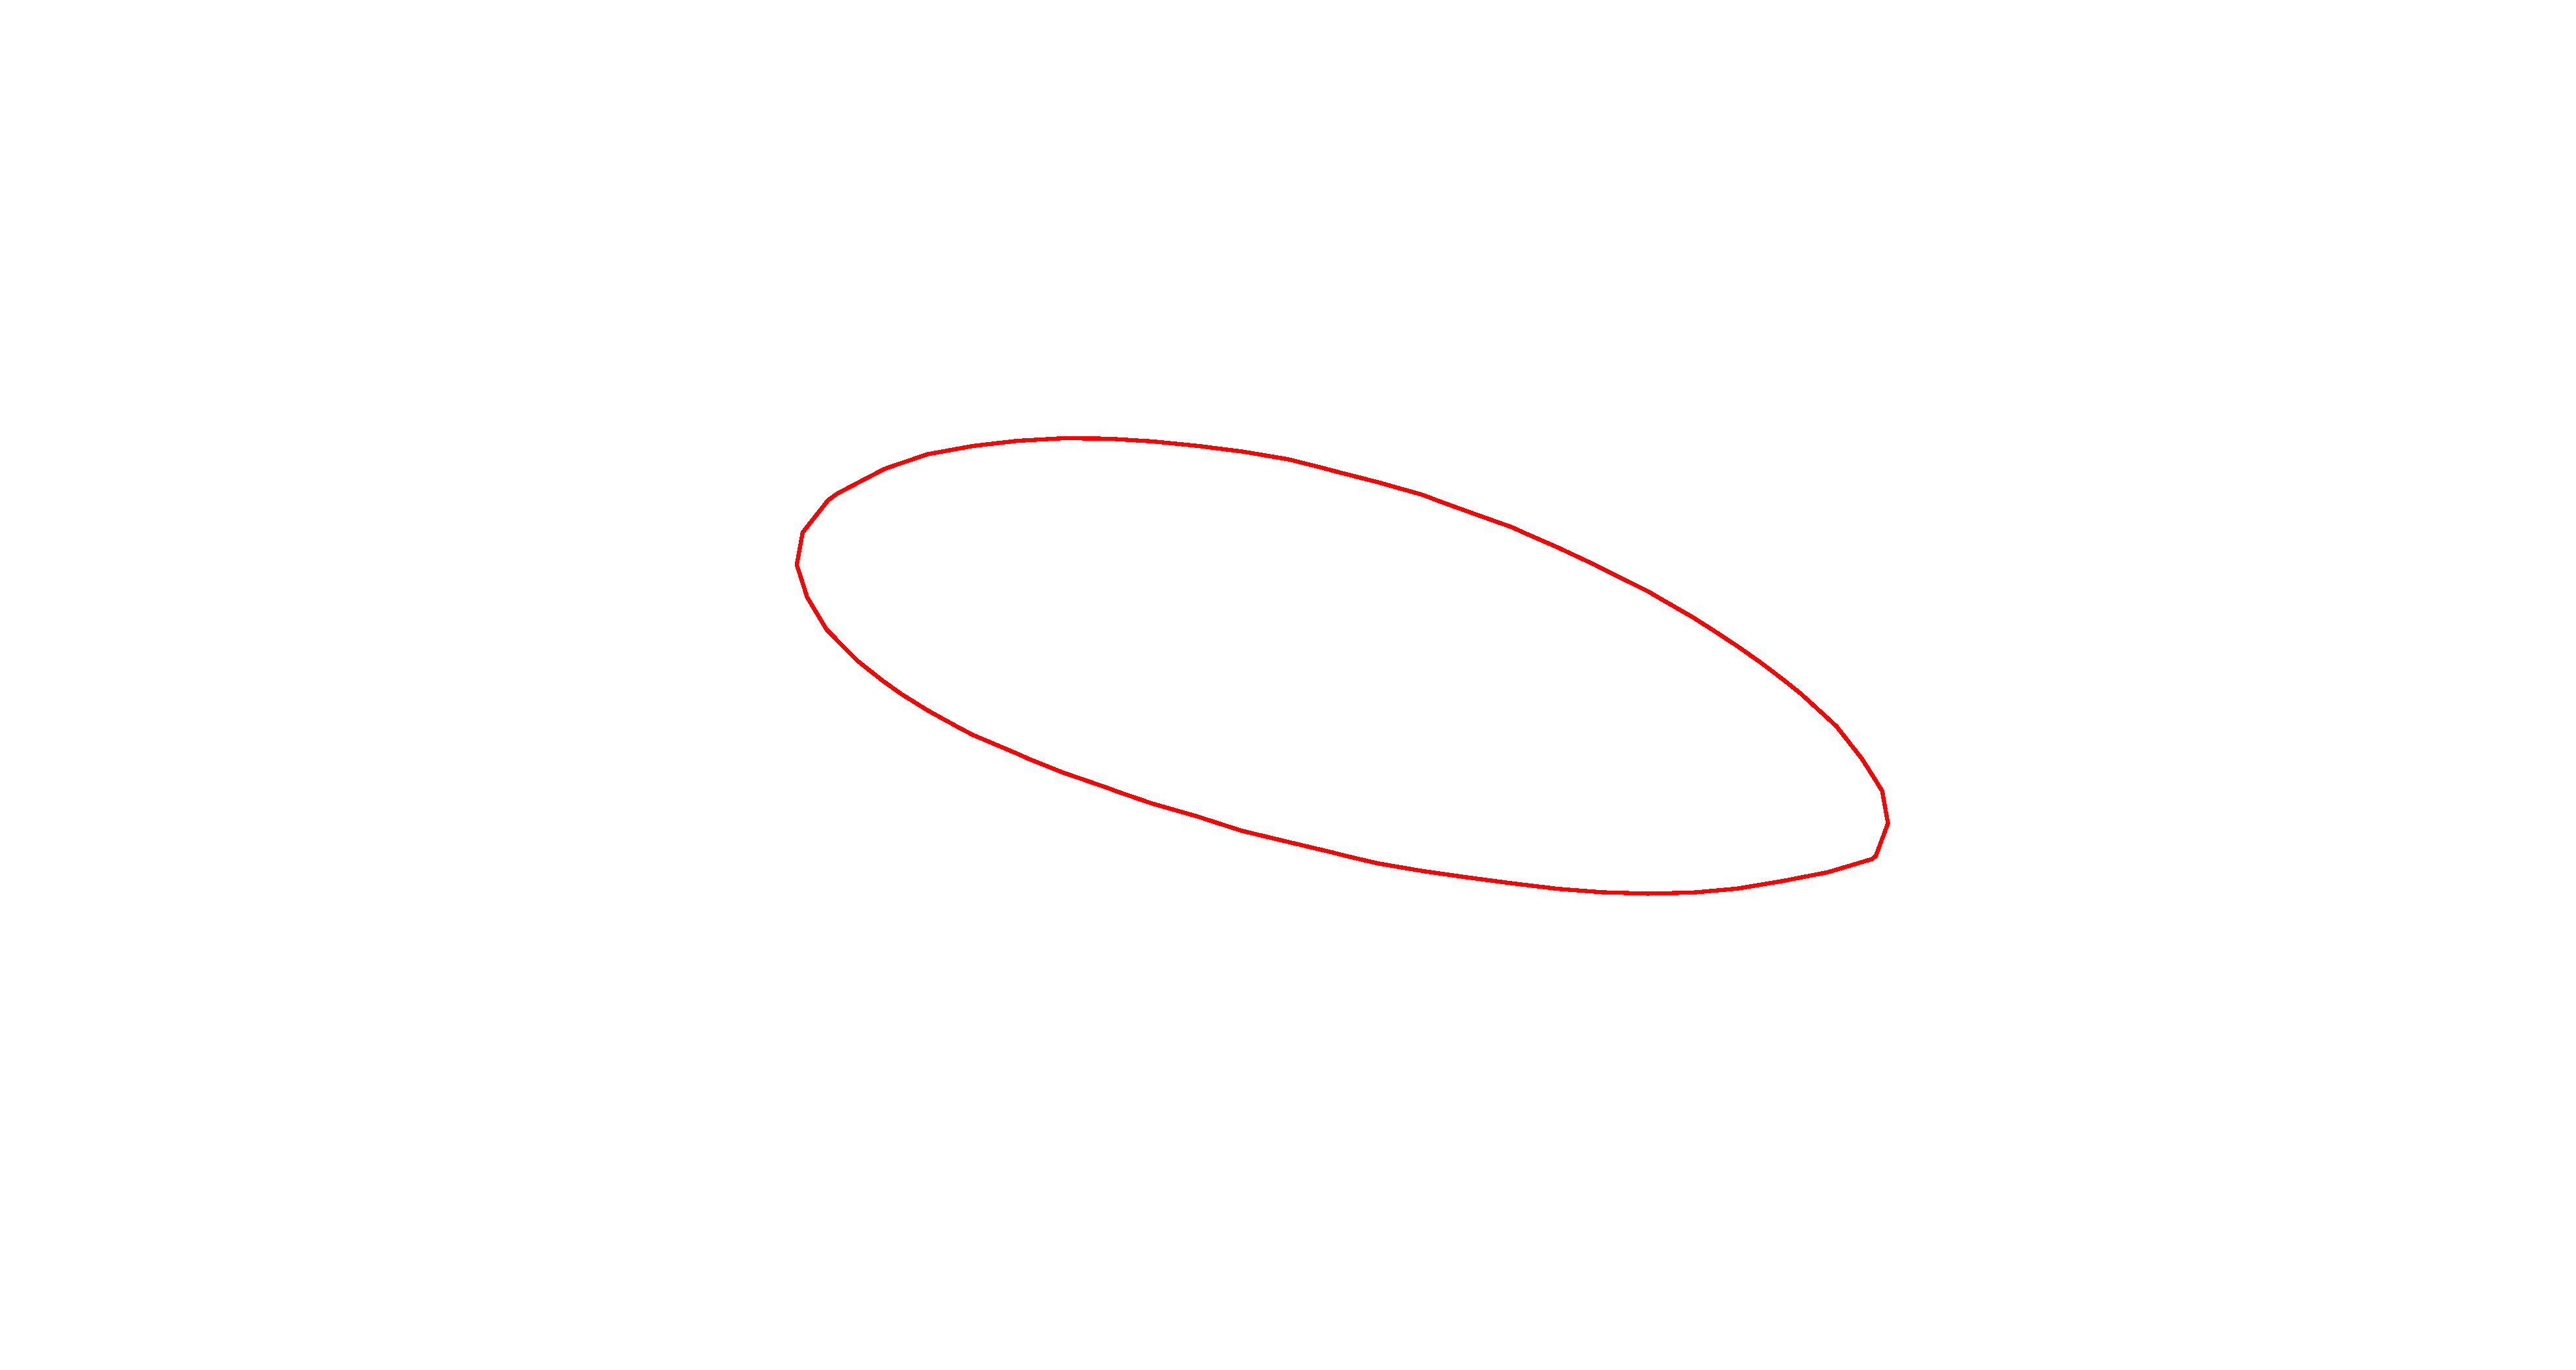
\includegraphics[scale=0.05,trim={10cm 10cm 8cm 10cm},clip]{C5.eps}$& 600
				%%%%%%%%%%%%%%%%%%%%%%%%%%%%%%%%%%%%%%%%%%%
				\\
				%%%%%%%%%%%%%%%%%%%%%%%%%%%%%%%%%%%%%%%%%%%
				\hline
				\hline
			\end{tabular}\label{Table1}
		\end{center}
	\end{table}
	%%%%%%%%%%%%%%%%%%%%%%%%%%%%%%%%%%%%%%%%%%%%%%%%%%%%%%
	%%%%%%%%%%%%%%%%%%%%%%%%%%%%%%%%%%%%%%%%%%%%%%%%%%%%%%
	%%%%%%%%%%%%%%%% Table 1 end %%%%%%%%%%%%%%%%%%%%%%%%%
	%%%%%%%%%%%%%%%%%%%%%%%%%%%%%%%%%%%%%%%%%%%%%
	
	
	The rising process of a bubble may exhibit different rise characteristics and flow dynamics depending on the non-dimensional parameters of the bubble, such as Reynolds and Bond numbers~\cite{Cano-Lozano2016, Hua2007}. In general, three types of rising paths were identified, including rectilinear, spiral, and straight rocking. In all cases in this study, the bubble deforms and reaches a steady-state shape during the rise process. Utilizing the computational setup as shown in figure~\ref{Fig1}(a) with SI-LSM$_{col}$, three cases of rising bubbles referred hereafter as C$_1$, C$_2$, and C$_3$ are considered for bubble deformations. Whereas, utilizing the computational setup as shown in figure~\ref{Fig1}(b) with CDI, two complex rising cases exhibiting three-dimensional characteristics referred to as C$_4$ and C$_5$ are simulated on a 3D \textit{Cartesian} coordinate system. Also, Table~\ref{Table1} shows the non-dimensional physical properties of the fluids for the present five cases simulated. Cases C$_1$--C$_3$ exhibit a straight rising path, while a more complex behavior, including a zigzag rise trajectory from an initial rectilinear path, is obtained in cases C$_4$ and C$_5$, making these two cases challenging for simulation and for the data-driven methods utilized here. Due to the periodic motion in the oscillatory region, data-driven methods are expected to perform more efficiently when applied only to this stage than in the case where the rectilinear part is also included. Thus, it is important to assume a generalized case where the analysis is not only restricted to the periodic behavior. Therefore, unlike previous studies that primarily focused on either the oscillatory~\cite{Yin2023} or rectilinear regions~\cite{Yin2023a} separately, the present work attempts to assess the entire duration of the rising process, including the rectilinear, transition, and oscillatory stages. 
	
	\section{Frame of reference}
	\label{Framework}
	The obtained flow fields from the simulation may be analyzed from different perspectives, including Eulerian, Lagrangian, and \hl{moving-Eulerian} frameworks. The gas volume fraction field representing the bubble's interface is illustrated in figure~\ref{Fig2} for case C$_3$ using the different frameworks at three time instances. As shown in figure~\ref{Fig2}(a) for the Eulerian framework, the observer focuses on the fixed grid points with varying flow properties in time. Instead, the Lagrangian framework, shown in figure~\ref{Fig2}(b), involves tracking the fluid elements from an initial condition; in this case, those in the Eulerian frame at the starting time. The position of a fluid element is described through the ordinary differential equation, given as
	
	%%%%%%%%%%%%%%%%%%%%%%%%%%%%%________Figure_2___________%%%%%%%%%%%%%%%%%%%%%%%%%
	\begin{figure}[!tpb]
		\centering
		
\includegraphics[scale=0.85,trim={1.5cm 6cm 0cm 5cm},clip]{Figure_2.pdf}
		\caption{Instantaneous deformation of the rising bubble at$\tau=0.10,\,4.25,\,8$ for case C$_3$ in the Eulerian, Lagrangian,and \hl{moving-Eulerian} frameworks.}
		\label{Fig2}
	\end{figure}
	%%%%%%%%%%%%%%%%%%%%%%%%%%%%%________Figure_2_end___________%%%%%%%%%%%%%%%%%%%%%
	
	\begin{align}
		\frac{d \mathbf{x}(t)}{d t} &= \mathbf{u}(\mathbf{x},t),
		\label{eq 1}
	\end{align}
	
	\noindent where $\mathbf{x}$ and $\mathbf{u}$ denote the position and velocity of the fluid particle at time $t$, respectively. \hl{It should be noted that the number of Lagrangian particles is identical to the grid size of the Eulerian frame, as the tracers were initialized from the Eulerian grid.} For the \textit{axisymmetric} coordinate system, the velocity field $\mathbf{u}$ is taken directly from the Eulerian solution to initialize the particles at $t_0$ at the corresponding Eulerian grid points. The updated particle position is then obtained by integrating Eq.~(\ref{eq 1}) using a first-order (linear) time-integration scheme, which provides a lower computational cost when tracking a large number of particles. \hl{At each new particle location, the fluid properties—including velocity and gas volume fraction—are interpolated from the Eulerian field. From physical intuition in multiphase flow, and in the absence of phase change or mass transfer, a particle inside the carrier or dispersed phase is expected to remain in that phase, and therefore no interpolation would ideally be required to determine its gas volume fraction. However, in the present framework the particles are treated as passive tracers whose motion is governed solely by the continuous velocity field. Because the velocity field does not impose a physical constraint that prevents tracers from crossing the interface, particles initialized close to the interface may move into the opposite phase during tracking. For this reason, interpolation of the gas volume fraction is required to avoid mislabeling particles as inside or outside the bubble.} It is worth noting that interpolation schemes are known to be a major source of numerical error in particle-tracking algorithms \cite{Majd2024a}. To balance accuracy and computational efficiency, fifth-order Lagrange interpolation is used for the gas volume fraction, while a linear interpolation scheme is employed for the velocity components. A brief sensitivity analysis supporting these choices is provided in Appendix~\ref{Append_A}. 
	
	In the \hl{moving-Eulerian} configuration, as shown in figure~\ref{Fig2}(c), a moving frame of reference is considered. The time-varying origin of the \hl{moving-Eulerian} coordinate system and the Region of Interest (ROI) size are defined to capture the temporal evolution of the bubble interface. In this study, the ROI size is considered as $0.75D\times 1.5D$ for the two-dimensional \textit{axisymmetric} coordinate system. In contrast, a size of $1.5D\times 1.5D \times 1.5D$ is considered for the three-dimensional \textit{Cartesian} coordinate system. Meanwhile, for the origin, the moving framework is anchored to the bubble centroid. Figure~\ref{Fig2}(c) shows this origin as a filled red circle bounded within a yellow-colored bordered ROI. There are some notable advantages of using the \hl{moving-Eulerian} framework. No interpolation is needed as it uses the DNS values of the Eulerian field, which enhances the precision. Meanwhile, it benefits from the localized properties of the flow because of its translational nature. Furthermore, it is computationally efficient compared to the Lagrangian approach, particularly in 3D problems. \hl{The dataset obtained from the trajectories of the moving grid points is temporally low-dimensional compared to that of fixed Eulerian grid points. More precisely, a fixed Eulerian probe records a highly fluctuating, high-dimensional time series, whereas the trajectories of a moving tracer yield a smoother, more correlated signal. In this sense, the Lagrangian dataset is effectively temporally low-dimensional compared to the Eulerian one. This characteristics of the Lagrangian approach reduces the temporal complexity associated with transient problems at the expense of having to reconstruct the coordinates of the moving data points.}
	
	\section{Data-driven modal decomposition methods}
	\label{Data-driven methods}
	Assuming a dataset of real value $d_{n_s}[m]$ with $n_{s}=n_{c}n_{x}n_{y}n_{z}$ number of sampling data in which, $n_{c}$ is number of components and $m$ is the number of collected snapshots, the input data matrix $\mathcal{D}\in R^{n_{s}\times m}$ for data-driven analysis is given by
	
	\begin{align}
		\mathcal{D} = \begin{bmatrix}
			d_{1}[1] & d_{1}[2] & \cdots & d_{1}[m] \\
			d_{2}[1] & d_{2}[2] & \cdots & d_{2}[m] \\
			\vdots & \vdots & \vdots & \vdots \\
			d_{n_s}[1] & d_{n_s}[2] & \cdots & d_{n_s}[m]
		\end{bmatrix}.\label{eq 2}
	\end{align}
	\noindent With the input data matrix~(\ref{eq 2}) established, the high-dimensional flow field data sets are decomposed using data-driven methods into low-dimensional spatiotemporal structures, so-called modes, representing the most dominant flow patterns. In general, decomposition techniques are categorized into energy and frequency-based methods. POD, as an energy-based method, and DMD, as a frequency-based method, are considered in this study. While these methods are closely linked and may represent similar flow characteristics when applied to a given dataset, a few differences make them unique for different purposes. For instance, both of these methods are known as ROMs and, therefore, can be applied to reconstruct the original data using only a few modes. POD and DMD are also known to be equation-free methods, meaning that they do not rely on the governing equations of the system. This allows them to be applied to numerical and experimental datasets.
	
	Regarding the discrepancies, only DMD can predict the system's future state when benefiting from ROMs. Each DMD mode is associated with a single frequency, while in the case of POD, there may be several frequencies related to multiple scales for one mode. With respect to reconstruction, POD is more straightforward since the extracted modes are arranged by energy in descending order. This facilitates the selection of the most relevant modes. In contrast, DMD reconstruction relies on the contribution of each mode's amplitude. A few criteria suggested to obtain the DMD amplitudes will be discussed further in section~\ref{DMD}.  
	
	
	\subsection{POD}
	\label{POD}
	
	This energy-based method can optimally extract the most energetic feature of the flow through dimensional reduction. In practice, one way of dimensional reduction is by taking the singular value decomposition (SVD) of $\mathcal{D}$, given as
	\begin{align}
		\mathcal{D} = \varphi \Sigma \psi^T ,\label{eq 3}
	\end{align}
	\noindent where $\varphi \in R^{n_s\times m}$ holds the spatial modes and $\psi\in R^{m\times m}$ contains the temporal ones. Note that in the SVD computation, $\Sigma\in R^{m\times m}$ is a diagonal matrix holding singular values of $\mathcal{D}$ in descending order, reflecting the importance of each mode. In most cases, $\mathcal{D}$ is a tall and skinny matrix with millions of rows and thousands of columns, making the SVD computation costly and impractical. An alternative approach is the method of snapshot proposed by \citet{Sirovich1987} by considering the right eigenvalue problem of the matrix $\mathcal{D}^T\mathcal{D}$ with a much smaller size of $m\times m$, given as 
	
	\begin{align}
		\mathcal{D}^T\mathcal{D}\psi _j = \lambda _j \psi _j.\label{eq 4}
	\end{align}
	
	\noindent By solving Eq.~(\ref{eq 4}) for eigenvalues $\lambda _j$ and their corresponding eigenvectors $\psi _j$, the spatial modes $\varphi _j$, with $j\in [1,~.~.~.~, m]$ are determined as
	
	\begin{align}
		\varphi _j = \mathcal{D} \psi _j \frac{1}{\sqrt{\lambda _j}}.\label{eq 5}
	\end{align}
	
	\noindent It should be noted that the singular values of the SVD decomposition in Eq.~(\ref{eq 3}) are related to the eigenvalues obtained in Eq.~(\ref{eq 4}) by $\mathcal{S}_j = \sqrt{\lambda_j}$. The method of snapshot has been used widely due to the smaller size of the correlation matrix. However, one may still use the SVD-based method, as it is reliable and accurate even in the presence of roundoff errors. POD modes are then ranked based on their energy level, which is given by the eigenvalues. Thus, incoherent noise with low energy levels appears in the higher-order modes.
	
	
	\subsection{DMD}
	\label{DMD}
	
	This decomposition technique is capable of identifying spatial features and their dynamics. Each mode is associated with a single frequency of oscillation and decay/growth given by the corresponding eigenvalues. Many mathematical formulations exist in the literature, amongst which the algorithm-1 in the work of \citet{H.Tu2014} is presented here. It involves four main steps, including
	\begin{itemize}
		\item[1.] The arrangement of input data matrices $\mathcal{D}'$ and $\mathcal{D}''\in R^{n_{s}\times m-1}$:
		\begin{subequations}\label{eq 6}
			\begin{align}
				\mathcal{D}' = \begin{bmatrix}
					d_{1}[1] & d_{1}[2] & \cdots & d_{1}[m-1] \\
					d_{2}[1] & d_{2}[2] & \cdots & d_{2}[m-1] \\
					\vdots & \vdots & \vdots & \vdots \\
					d_{n_s}[1] & d_{n_s}[2] & \cdots & d_{n_s}[m-1]
				\end{bmatrix}, \label{eq 6a} \\
				\mathcal{D}'' = \begin{bmatrix}
					d_{1}[2] & d_{1}[3] & \cdots & d_{1}[m] \\
					d_{2}[2] & d_{2}[3] & \cdots & d_{2}[m] \\
					\vdots & \vdots & \vdots & \vdots \\
					d_{n_s}[2] & d_{n_s}[3] & \cdots & d_{n_s}[m]
				\end{bmatrix}.\label{eq 6b}
			\end{align}
		\end{subequations}
		\item[2.] Computing the truncated SVD by considering only a reduced $r$ number of modes:
		\begin{align}
			\mathcal{D}' = U_r\Sigma _r W_r^T, \label{eq 7}
		\end{align}
		\item[3.] Solving the eigenvalue problem of:
		\begin{align}
			\tilde{A} \tilde{v_j} = \gamma_j \tilde{v_j}, \label{eq 8}
		\end{align}
		where $\tilde{A}=U_r^T \mathcal{D}'' W_r \Sigma_r^{-1}$. The non-zero eigenvalue $\gamma_j= a + ib$ obtained in Eq.~(\ref{eq 8}) is a complex number. The real and imaginary parts represent the growth/decay rate and the frequency of oscillation corresponding to each mode, respectively.
		
		\item[4.] Determining the spatial modes as follows:
		\begin{align}
			\varphi _j = U_r\tilde{v_j}. \label{eq 9}
		\end{align}
		
	\end{itemize}
	It is important to note that, unlike POD, where the importance of the modes is characterized based on their energy content (eigenvalues), the DMD modes are typically ranked based on their amplitudes. There are different techniques to obtain the DMD amplitudes that are discussed in the following sections.
	
	
	\subsubsection{DMD amplitudes}
	\label{DMD amplitudes}
	The reconstruction procedure in DMD requires determining the amplitudes corresponding to each DMD mode. The most straightforward but less accurate approach is to compute the initial amplitudes as follows \cite{Kutz2016}
	
	\begin{align}
		d(t)\approx \sum_{j=1}^{m} \varphi_j e^{\omega_j t} b_j = \boldsymbol{\varphi}~exp (\boldsymbol{\Omega} t)\boldsymbol{b}.
		\label{eq 10}
	\end{align}
	
	\noindent where $d(t)$ is the reconstructed data sequence, $t=k\Delta t$, $k=0, 1, ..., m-2,m-1$, $\Delta t$ is a constant time interval, $\omega _j = log(\gamma_j)/\Delta t$ are the diagonal entries of $\Omega$, and $\boldsymbol{b} = \boldsymbol{\varphi^{\dagger}} d[0]$ are the initial amplitudes. Note that the superscript $\dagger$ denotes the Moore-Penrose pseudoinverse. These amplitudes reflect the importance and relevance of each mode to the overall dynamic of the system. Therefore, one may assume that only DMD modes with the highest amplitudes should be included in the reconstruction. Since the amplitudes are obtained by projecting the first snapshot onto the DMD modes, the reconstruction is more likely accurate for early-stage flow features. This might also lead to incomplete reconstruction for cases with structures that become more important as the system evolves. 
	
	An alternative approach to obtain the DMD amplitudes involves solving an optimization problem, where a trade-off is made between the sparsity of the included modes and the accuracy of the reconstruction. This strategy, proposed by \citet{Jovanovic2014}, can efficiently retain the most relevant modes with their actual amplitudes by solving the optimization problem $min~||\boldsymbol{\mathcal{D}'} - \boldsymbol{\varphi} \boldsymbol{B_b} V_\gamma||_F^2$. Where $\boldsymbol{B_b}$ is the diagonal matrix of amplitude vector $\boldsymbol{b} = [b_1,  b_2,~...~,b_j]$ and $V_\gamma$ is the Vandermonde matrix containing the eigenvalues of $\tilde{A}$.  Using SVD properties, the definition of matrix $\varphi$, and some algebra, the result is then in a quadratic form that is solved using the alternating direction method of multipliers technique. Readers are referred to previously published literature \cite{Jovanovic2014,Schmid2023} for more details on this method. 
	
	
	%%%%%%%%%%%%%%%%%%%%%%%%%%%%%________Figure_3___________%%%%%%%%%%%%%%%%%%%%%
	\begin{figure}[!t]
		\centering
		
\includegraphics[scale=0.6,trim={0cm 2.4cm 0cm 0cm},clip]{Figure_3.pdf}
		\caption{Relative reconstruction error for the velocity and gas volume fraction fields in Eulerian, Lagrangian, and \hl{moving-Eulerian} frameworks for the rising bubble a) case C$_1$ and b) case C$_3$. Red, blue, and green colors correspond to the Eulerian, Lagrangian, and \hl{moving-Eulerian} frameworks, while the dashed and solid lines refer to DMD and POD techniques, respectively. Squares and triangles denote the gas volume fraction and velocity fields.}
		\label{Fig3}
	\end{figure}
	%%%%%%%%%%%%%%%%%%%%%%%%%%%%%________Figure_3_end___________%%%%%%%%%%%%%%%%%
	
	
	
	\section{Results and discussion}
	\label{Results and discussion}
	
	Different observation values may be considered to train data-driven algorithms depending on the property being studied. For instance, the gas volume fraction is used to characterize the bubble deformation, track the bubble interface, and estimate the rising trajectory. On the other hand, one may apply data-driven techniques to the velocity field to gain insights into the dynamics and spatiotemporal structures in the bubble's wake. Both the gas volume fraction and velocity field are required for more complex rise properties such as the terminal velocity. 

	Observation values can be used in data-driven algorithms from the Eulerian and Lagrangian perspectives. \hl{For brevity, the framework and the observation values are abbreviated as $\textit{E}$, $\textit{L}$, and $\textit{\hl{ME}}$ for Eulerian, Lagrangian, and \hl{moving-Eulerian} frameworks, followed by $\textit{G}$, $\textit{V}$ or $P$ which refer to gas volume fraction, upward component of the velocity field, and the coordinates of the data points, respectively. Here, only the upward (vertical) velocity component is used, as the rise velocity is determined exclusively by this component. Considering three frame of references, two decomposition methods and three observation values, there can be 18 combinations that can be defined. For instance, the decomposition of the upward velocity field in the Eulerian frame using the POD method is denoted as $\textit{EV-POD}$. Further details regarding the input and output data matrices are given in Appendix B.}
	
	\subsection{Reconstruction error of observation value}
	\label{Reconstruction error analysis}
	In this section, different flow variables, including velocity field and gas volume fraction, are reconstructed using POD and DMD methods in Eulerian, Lagrangian, and \hl{moving-Eulerian} frameworks. The accuracy of the reconstructed field is evaluated by means of the Frobenius norm of the difference between the original input data matrix and its approximation. Using the properties of SVD, the relative reconstruction errors of a field using POD and DMD for $r$ number of modes are simplified and given by:
	
	\begin{subequations}\label{eq 12}
		\begin{align}
			R_{err}(r)_{_{POD}} = \frac{||\mathcal{D} - \mathcal{D}_r||_F^2}{||\mathcal{D}||_F^2} = \frac{\sum\limits_{j=r+1}^m \mathcal{S}_j^2}{\sum\limits_{j=1}^m\mathcal{S}_j^2}, \label{eq 12a} \\
			R_{err}(r)_{_{DMD}} = \frac{||\mathcal{D}' - \varphi B_r V_{\gamma}||_F^2}{||\mathcal{D}'||_F^2} = \frac{||\Sigma W^T-\tilde{v_j} B_r V_{\gamma}||_F^2}{||\Sigma W^T||_F^2}.\label{eq 12b}
		\end{align}
	\end{subequations}
	
	\noindent The above errors in the reduced space are computationally less expensive than working with the full input data matrix of size $n_s \times m$. Preceding the discussion on the efficiency of each method, it is necessary to emphasize that two types of errors are assessed in this study. One is already introduced in Eqs.~(\ref{eq 12}), while the other is the conventional root mean square deviation (RMSD) used for scalar variables. The former is used for the overall evaluation of the reconstructed field. In contrast, the latter is applied to quantitative time-varying parameters such as the rise velocity and circularity of the bubble, which will be discussed further in section~\ref{Bubble interface}.
	
	The error of reconstructed fields is evaluated using Eqs.~(\ref{eq 12}) in the Eulerian, Lagrangian, and \hl{moving-Eulerian} frameworks using POD and DMD techniques as shown in figures~\ref{Fig3}(a) and \ref{Fig3}(b) for cases C$_1$ and C$_3$, respectively. The former exhibits the least deformation, and the latter exhibits the most deformation. Considering the results of the bubble C$_1$ with small deformation in figure~\ref{Fig3}(a), the relative reconstruction error of POD converges to zero more rapidly than DMD in Eulerian, Lagrangian, and \hl{moving-Eulerian} frameworks, highlighting the greater efficiency of POD compared to DMD. With the gas volume fraction as the primary variable, EG-DMD and EG-POD require 89 and 17 modes to achieve the relative reconstruction error of approximately 5.6\% . See the dashed and solid red lines with square markers representing the gas volume fraction field. The most accurate results are achieved with LG-POD and SLG-POD, where the relative reconstruction error is as small as 0.065\% and 0.075\% with 10 modes, respectively. In the case of LG-DMD and SLG-DMD, the relative reconstruction errors are approximately 3.1\% and 6.5\% with 10 modes, respectively. The analysis of the relative reconstruction error for the bubble C$_3$ shown in figure~\ref{Fig3}(b) supports the established patterns for C$_1$. However, due to the greater deformation in this case, a higher relative reconstruction error is observed with the same number of modes compared to case C$_1$ with smaller deformation. This can be observed for SLG-POD and LG-POD schemes with the relative reconstruction errors of 2.2\% and 0.3\% with 10 modes, respectively. Similar observations are noted in the case of the velocity field for C$_1$ and C$_3$. However, it is less dispersed and requires fewer modes for accurate reconstruction compared to the gas volume fraction in the Eulerian and \hl{moving-Eulerian} frameworks. For example, the relative reconstruction error for the velocity field in C$_3$ is approximately 1.2\% and 0.2\% for EV-POD and SLV-POD when only 10 modes are used. Overall, based on the analysis of the relative reconstruction error, one may conclude that the Lagrangian, \hl{moving-Eulerian}, and Eulerian frameworks yield results in descending order of accuracy.
	
	\subsection{Bubble interface}
	\label{Bubble interface}
	An overall analysis of the relative reconstruction error shows that data-driven techniques perform more efficiently in the \hl{moving-Eulerian} and Lagrangian frameworks. However, their accuracy in approximating the bubble interface and rise properties has not been precisely examined. To address this, the bubble interface, its rise velocity, and circularity are approximated for C$_1$, C$_2$, and C$_3$ using 10 modes during the rising process. The truncation rank of 10 is selected based on the cumulative energy given in Eq.~(\ref{eqB1}) for the three-dimensional case C$_5$ as the most complex case in the present work (see Appendix~\ref{Append_B}). 
	
	Circularity, as a quantitative geometric metric, provides a precise criterion to assess the accuracy of the reconstructed bubble shape~\cite{Hysing2009}. A value of 1 corresponds to a perfectly circular bubble, while lower values indicate deformation. However, in this study, circularity alone proves insufficient due to irregular shapes and discontinuities in the noisy reconstructed fields. This issue is particularly pronounced in the Lagrangian framework, where multiple shape variations and noise lead to large fluctuations—and in some cases, discontinuities—in the circularity profile (see L-DMD in figures~\ref{Fig4}, \ref{Fig5}(b), \ref{Fig5}(d), and \ref{Fig5}(f)). Therefore, to gain a more reliable assessment, the reconstructed bubble interface over time shown in figure~\ref{Fig4} is evaluated alongside the temporal variation of circularity in figures~\ref{Fig5}(b), \ref{Fig5}(d), and \ref{Fig5}(f).
	
	%%%%%%%%%%%%%%%%%%%%%%%%%%%%%________Figure_4___________%%%%%%%%%%%%%%%%%%%%%
	\begin{figure}[!tpb]
		\centering
		
\includegraphics[scale=0.81,trim={2.7cm 3cm 2.1cm 1cm},clip]{Figure_4.pdf}
		\caption{Bubble deformation using 10 modes for cases a) C$_1$, b) C$_2$, and c) C$_3$. Results are mirrored about $Z=0$ and shown at $\tau = 0.07,~3.36,~4.65,~9.94,~13.22,~16.51,~19.80,~23.09$. For clarity, each snapshot is offset by $0.025D$ in the axial direction. Yellow solid and red dashed lines denote reconstructed and DNS iso-contours of the gas volume fraction 0.5, respectively.}
		\label{Fig4}
	\end{figure}
	%%%%%%%%%%%%%%%%%%%%%%%%%%%%%________Figure_4_end___________%%%%%%%%%%%%%%%%%%%%%
	
	As illustrated in figures~\ref{Fig4}(a) and \ref{Fig4}(b), despite high relative reconstruction errors of 83.06\% and 90.9\% for C$_1$ and C$_2$, some faint representation of the bubble is detected when E-DMD is applied. As shown in figure~\ref{Fig4}(c) for C$_3$, E-DMD fails in reconstructing the bubble interface due to the shape complexities. E-POD, on the other hand, can capture the overall deformation of the bubble during the rise process with the relative reconstruction error of 10.97\%, 15.85\%, and 28.97\% for C$_1$, C$_2$, and C$_3$, respectively. This highlights the greater efficiency of POD over DMD in the Eulerian framework. Having said that, one may notice the shape distortions and a phase lag relative to DNS for E-POD. In the case of C$_1$, for example, the bubble interface is approximated about 0.25D above the interface obtained in DNS as shown in figure~\ref{Fig4}(a). Furthermore, shape distortions causing errors in the interface may be reflected in the circularity profile, as it exhibits deviations with some oscillations. For instance, the circularity profile of C$_1$ in figure~\ref{Fig5}(b) exhibits discrepancies from the DNS with an RMSD error of 3\%. In a more complex case of C$_3$ with more deformation shown in figure~\ref{Fig4}(c), the initial and terminal shapes of the bubble are captured, while the intermediate stages show a fragmented bubble. This can be clearly observed in the circularity profile of E-POD in figure~\ref{Fig5}(f), where large deviations are observed at $5 < \tau < 23$. As a final point, the efficiency of data-driven methods decreases as the bubble exhibits greater deformation in the Eulerian framework. 
	
	The bubble interface is more accurately reconstructed in the Lagrangian framework, though shape distortion and artifacts still exist. As shown in figure~\ref{Fig4}, the shape distortion, more pronounced in L-DMD, could be misinterpreted as bubble breakage. A similar false feature is observed in L-POD, though it is less significant than in L-DMD. These shape irregularities may account for large fluctuations and discontinuities observed in the circularity profile of Lagrangian methods in figures~\ref{Fig5}(b), \ref{Fig5}(d), and \ref{Fig5}(f). Interestingly, L-POD maintains a smoother and more consistent profile with less pronounced fluctuations than L-DMD. The noisy and distorted bubble shape in the Lagrangian framework is primarily due to the scattered output of the particle tracking process. Since the field of interest is represented by interpolating the scattered data of particle tracking, it may lack sufficient resolution near the axisymmetric boundary, and the bubble interface is not detected in that region, leading to false breakage and noisy results. This shortcoming of the Lagrangian approach was previously reported by \citet{Haller2011} for computing the forward Finite-time Lyapunov exponent (FTLE) field at the final position of the particle trajectories. Recognizing this limitation, the relative reconstruction errors for C$_1$, C$_2$, and C$_3$ using L-DMD are 3.15\%, 4.8\%, and 7.7\%, respectively, whereas for L-POD, they are 0.088\%, 0.13\%, and 0.29\%. Clearly, the relative reconstruction error is much lower in the Lagrangian framework than in the Eulerian framework. However, one may argue that these small errors calculated using Eqs.~(\ref{eq 12}) are inconsistent with the results in figures~\ref{Fig4} and \ref{Fig5}. In other words, a lower relative reconstruction error should yield a bubble with less shape distortion or artifacts. This discrepancy can be explained by the fact that Eqs.~(\ref{eq 12}) only reflect the errors of the data-driven techniques since they measure the difference between the input $\mathcal{D}$ and reconstructed $\mathcal{D}_r$ matrices. Thus, the error associated with Lagrangian tracking, which leads to false diagnoses of bubble breakage, is not incorporated. Finally, the results of L-POD and L-DMD align with the findings in the previous section, further emphasizing the superior efficiency of POD compared to DMD.
	
	For \hl{moving-Eulerian} framework as shown in figures~\ref{Fig4}(a) and \ref{Fig4}(b), the bubble interface is accurately reconstructed at $\tau >9.94 $ for C$_1$ and $\tau >13.2 $ for C$_2$ when \hl{ME}-DMD is used. However, the reconstruction lacks accuracy in the early stages, resulting in bubble distortion. Analogously shown in figures~\ref{Fig5}(b) and \ref{Fig5}(d), the circularity profile of \hl{ME}-DMD shows a large deviation in the early stages of the rise and later aligns with DNS at $\tau \approx 15$. Accordingly, the relative reconstruction error of \hl{ME}-DMD is 6.47\% and 11.7\% for the bubbles C$_1$ and C$_2$, respectively, with the largest contributions occurring in the early stages. For C$_3$, as shown in figure~\ref{Fig4}(c), the reconstruction fails with an error of approximately 54\% when \hl{ME}-DMD is applied. Thus, one may infer that the DMD is not reliable and accurate when applied in the \hl{moving-Eulerian} framework for complex cases. Even in the case of simple bubbles with small deformation, the bubble interface is not accurately determined in the early stages. This can be observed in the circularity profile of C$_1$ and C$_2$ in figures~\ref{Fig5}(b) and~\ref{Fig5}(d). In contrast, \hl{ME}-POD accurately captures the bubble interface throughout the rise process, including the early stages and terminal state. The relative reconstruction error of this method is 0.1\%, 0.36\%, and 2.2\% for C$_1$, C$_2$, and C$_3$, respectively. Such consistency throughout the rising process can be clearly observed in the circularity profile of \hl{ME}-POD in figures~\ref{Fig5}(b), \ref{Fig5}(d), and \ref{Fig5}(f). The RMSD errors are approximately 0.11\%, 0.78\%, and 3\% for cases C$_1$, C$_2$, and C$_3$, respectively. Overall, the above discussion may suggest that \hl{ME}-POD exhibits the most accurate interface with no noticeable artifacts for the cases considered in this work while maintaining high efficiency and low computational cost.
	
	\subsection{Rise velocity}
	\label{Rise velocity}
	
	%%%%%%%%%%%%%%%%%%%%%%%%%%%%%________Figure_5___________%%%%%%%%%%%%%%%%%%%%%
	
	\begin{figure}[!tpbh]
		\centering
		
\includegraphics[scale=0.79,trim={0cm 1.0cm 0cm 1.5cm},clip]{Figure_5.pdf}
		\caption{Rise velocity (Left) and circularity (Right) approximated using 10 modes for the rising bubble case (a-b) C$_1$, (c-d) C$_2$, and (e-f) C$_3$. The same number of modes is used for the velocity and gas volume fraction fields.}
		\label{Fig5}
	\end{figure}
	
	%%%%%%%%%%%%%%%%%%%%%%%%%%%%%________Figure_5_end___________%%%%%%%%%%%%%%%%%%%%%
	
	A widely analyzed output parameter associated with rising bubbles is their rise velocity, known as the terminal velocity, once a steady state is reached. In this work, the rise velocity of the bubble is defined as the mean velocity of its center of mass as it rises through initially stagnant fluid, calculated by spatially averaging the velocity component in the direction opposite to the gravitational vector within the bubble~\cite{Hysing2009}. Two observation fields, the velocity component in the axial direction and the gas volume fraction, are required to calculate the rise velocity. The gas volume fraction is used to identify the bubble interface and the corresponding grid points/particles. The velocity field is used to compute the rise velocity at the identified grid points/particles. Thus, simultaneously, the estimated rise velocity might be subject to errors from the reconstructed velocity and gas volume fraction fields. As previously shown in section~\ref{Reconstruction error analysis}, for the Eulerian and \hl{moving-Eulerian} frameworks, the relative reconstruction error of the velocity field is much lower than the gas volume fraction. Therefore, it is worth examining the effect of inaccuracy in the gas volume fraction field when estimating the rise velocity. To this end, the variation of the bubble's circularity over time is monitored alongside the rise in velocity. This analysis provides insights into how an inaccuracy in the gas volume fraction influences the rise velocity. 
	
	The time variation in rise velocity, obtained using different methods, are compared to DNS for the three cases C$_1$, C$_2$, and C$_3$ as shown in figures~\ref{Fig5}(a), \ref{Fig5}(c), and \ref{Fig5}(e), respectively. It should be noted that the methods incapable of identifying the interface in section~\ref{Bubble interface} are excluded here. In particular, E-DMD and \hl{ME}-DMD for C$_3$, as well as E-DMD for C$_1$ and C$_2$ are not considered. In the case of C$_1$ with less deformation shown in figure~(\ref{Fig5})(a), E-POD provides accurate results for the rising velocity with the RMSD error of 1.5\%. Nevertheless, it exhibits low-amplitude oscillations, particularly at $\tau >18$. As shown in figures~\ref{Fig5}(c) and \ref{Fig5}(e) for cases C$_2$ and C$_3$ with more complexity, E-POD becomes less accurate with the RMSD error of 5.6\% and 26\%, respectively. Notably, the slight low-amplitude oscillations in E-POD observed in rise velocity profiles of cases C$_1$ and C$_2$ might be linked to the similar oscillations observed in their corresponding circularity profiles, highlighting the effect of shape distortion on the estimation of rise velocity. In the Lagrangian approach, data-driven techniques deviate significantly from the DNS values and produce unacceptably large errors, primarily due to the particle-to-grid interpolation errors. As explained in Appendix~\ref{Append_A}, using a linear interpolation function for the gas volume fraction results in a significantly less accurate rise velocity. On the other hand, the \hl{moving-Eulerian} framework provides an accurate estimation of the rise velocity. Using \hl{ME}-POD, the RMSD errors for cases C$_1$, C$_2$, and C$_3$ are estimated to be 0.1\%, 0.3\%, and 3\%, respectively. Nevertheless, \hl{ME}-DMD deviates early on and during the transition stage ($\tau$ < 15) but aligns with the DNS at the terminal velocity. As shown for \hl{ME}-DMD in figure~\ref{Fig5}(b), a similar trend is observed for the circularity, where the bubble resembles the terminal shape at early stages ($\tau < 15$) and becomes more aligned with DNS later. Thus, one may conclude that the corresponding errors in the shape can influence the rise velocity value. Furthermore, similar relations between the circularity and rise velocity can be found. For instance, the rise velocity and circularity profiles obtained via \hl{ME}-DMD deviate in the early stages and later align with DNS at $\tau \approx 12$. 
	
	Finally, considering the limitations of interpolation functions causing the large deviation from the DNS values and the high cost of tracking in the Lagrangian approach, as well as the poor performance of the data-driven methods in the Eulerian framework, one may infer that the \hl{moving-Eulerian} framework offers a balance between accuracy and computational cost. Consequently, the following section conducts further analyses of the 3D cases using the \hl{moving-Eulerian} framework.
	
	\subsection{3D cases of a rising bubble}
	
	The last and perhaps the most complex scenarios considered in this work are the 3D cases, C$_4$ and C$_5$, of a rising, deforming bubble with rectilinear, transition, and oscillatory stages. The \hl{ME}-POD and \hl{ME}-DMD schemes are considered for reconstructing the rise trajectory and bubble interface for these case. In case C$_4$, 10 modes are used for both properties whereas in C$_5$, 10 modes are used for the rise trajectory and 15 modes for the bubble interface. See figures~\ref{Fig6}(a) and \ref{Fig6}(b). Additionally, the rise velocity and sphericity of the bubble in 3D space are obtained, and the results are shown in figure~\ref{Fig7}. A similar discussion for a 2D bubble in Section~\ref{Bubble interface} will be presented here for a 3D bubble.
	
	%%%%%%%%%%%%%%%%%%%%%%%%%%%%%________Figure_6__________%%%%%%%%%%%%%%%%%%%%%
	\begin{figure}[!tpb]
		\centering
		
\includegraphics[scale=0.99,trim={4cm 8.5cm 4cm 1.5cm},clip]{Figure_6.pdf}
		\caption{Rise trajectory and the 3D bubble interface at three intervals $\tau_{1}-\tau_{3}$ for cases (a) C$_4$ with 10 modes and (b) C$_5$ with 15 modes for interface and 10 modes for trajectory using ME-POD and ME-DMD schemes. The red dashed line, green solid line, and blue dash-dotted line denote the corresponding rise property obtained via DNS, ME-POD, and ME-DMD, respectively.}
		\label{Fig6}
	\end{figure}
	%%%%%%%%%%%%%%%%%%%%%%%%%%%%%________Figure_6_end___________%%%%%%%%%%%%%%%%%%%%%
	
	
	In the case of C$_4$ with less deformation in the left-hand-side of figure~\ref{Fig6}(a), the rising trajectory, shown as a green solid line, is reconstructed using as few as 10 out of 490 modes with the \hl{ME}-POD scheme, aligning perfectly with the DNS values depicted as a red dashed line. Similarly, using the same number of modes with the \hl{ME}-DMD shown as a blue solid line, the reconstructed trajectory closely matches the DNS, with only minor deviations. The bubble's shape in 3D orientation and the corresponding 2D projection are shown on the right-hand side of figure~\ref{Fig6}(a). In this figure, the bubble's shape from DNS and its corresponding interface are depicted as a contour plot and red dashed line in the $x-y$ plane at three different instances during the rise process. The bubble interface determined via the \hl{ME}-POD is shown as a green solid line and perfectly coincides with the DNS data, while \hl{ME}-DMD, shown in a blue dashed line, struggles to capture the bubble interface accurately. Accordingly, the relative reconstruction errors of the interface are 0.14\% and 1.17\% using \hl{ME}-POD and \hl{ME}-DMD, respectively. The time variation of the sphericity profile is shown in figure~\ref{Fig7}(b) for C$_4$, confirming the accuracy of the methods. Similar to the observations in the 2D case, \hl{ME}-DMD exhibits deviations from DNS during the early stages of the rise and improves later in the oscillatory region. For further investigation, the number of modes used in \hl{ME}-DMD is increased to 28. The results indicate that increasing the number of modes to 28 improves the results of \hl{ME}-DMD, although it is not as accurate as \hl{ME}-POD with 10 modes. Accordingly, the RMSD errors of sphericity using \hl{ME}-POD with 10 modes and \hl{ME}-DMD with 28 modes are 0.18\% and 0.65\%, respectively. In the case of C$_5$ with more complexity in deformation shown in figure~\ref{Fig6}(b), the rising trajectory is accurately reconstructed with 10 modes regardless of the methods. However, \hl{ME}-POD requires 15 modes to accurately capture the interface of the bubble with a relative reconstruction error of 0.41\%. \hl{ME}-DMD demonstrates relatively poor accuracy with a relative reconstruction error of 6.5\% using 15 modes. The time variation of sphericity for C$_5$ is shown in figure~\ref{Fig7}(d) highlighting the efficiency of different methods. \hl{ME}-POD accurately detects the bubble deformation throughout the rising process, while \hl{ME}-DMD demonstrates large errors, particularly during the early stages. Further investigation of \hl{ME}-DMD with 30 modes reveals that despite improvements in the results, the error continues to be higher than \hl{ME}-POD. In particular, the RMSD error of sphericity is 0.85\% and 3.2\% using \hl{ME}-POD with 15 and \hl{ME}-DMD with 30 modes, respectively. Observations from case C$_5$, which exhibits complex deformation, suggest that the efficiency of data-driven techniques decreases and that a greater number of modes is required when applied to a 3D bubble with complex deformation. However, this reduction is not significant for \hl{ME}-POD, as it requires only five additional modes compared to C$_4$ with 10 modes. 
	
	The rise velocity of the 3D bubbles C$_4$ and C$_5$ are estimated and compared with the DNS values. As illustrated in figures~\ref{Fig7}(a) and \ref{Fig7}(c), the rise velocity results are represented by red for DNS, green for \hl{ME}-POD, and blue for \hl{ME}-DMD. In the case of C$_4$, the rise velocity obtained via \hl{ME}-POD with 10 modes perfectly aligns with DNS values throughout the rising process from rectilinear to oscillatory. In contrast, \hl{ME}-DMD fails to provide correct results during the rectilinear and transition stages. The oscillatory behavior of the rise velocity is slightly detected using \hl{ME}-DMD, though it exhibits large deviations compared to the DNS data. The accuracy is improved in the transition and oscillatory stages, though the rectilinear part is still poorly reconstructed when 28 modes are used. Accordingly, the RMSD error of rise velocity is 4.9\% for \hl{ME}-POD. Considering the more complex 3D case C$_5$, \hl{ME}-POD with 15 and \hl{ME}-DMD with 30 modes approximate rise velocity with respective RMSD errors of 4.1\% and 16.4\%. Regarding the effect of shape inaccuracies on the rise velocity, one may notice the gradual improvement of accuracy in the rise velocity with a more accurate sphericity profile over time. Even though both schemes can accurately approximate global properties such as rise trajectory, \hl{ME}-POD yields more accurate results when it comes to local properties such as bubble interface and rise velocity.

	Overall, considering the results presented in this study, \hl{ME}-POD appears to be a promising scheme for capturing the dynamics of the bubble. \hl{In particular, the rise characteristics of the 3D bubble $C_5$, as the most complex case with 600 snapshots, were estimated using 15 modes, yielding a compression ratio of 40. This is notably less than the number of modes used by \citet{Yin2023a}, who employed 30 modes to represent 140 snapshots, resulting in a compression ratio of approximately 4.6.} The application of data-driven techniques in a \hl{moving-Eulerian} framework tackles the limitations of capturing transient phenomena while avoiding the particle-to-grid interpolation errors present in the Lagrangian approach. Furthermore, although \hl{ME}-DMD provides high accuracy in approximating the rise trajectory, it is not as accurate as \hl{ME}-POD for estimating the rise velocity and the interface for the 3D bubble, especially during the early stages of the rise.
	
	
	\section{Summary and conclusions}
	\label{Conclusion}
	
	
	The present work has examined the applicability of data-driven methods as a reduced-order model tool for state estimation of a rising bubble within different frameworks. Two in-house multiphase solvers, SI-LSM$_{\text{col}}$ on \textit{axisymmetric} coordinate system and CDI on 3D \textit{Cartesian} coordinate system, were used to obtain the flow field datasets of five cases for the training of the data-driven techniques. POD and DMD with optimized amplitude were applied within the Eulerian, Lagrangian, and \hl{moving-Eulerian} perspectives. The evaluation criteria focused on the relative reconstruction error of the observation fields and the RMSD of key rising characteristics such as circularity, rise trajectory, and rise velocity. 
	
	%%%%%%%%%%%%%%%%%%%%%%%%%%%%%________Figure_7__________%%%%%%%%%%%%%%%%%%%%%
	\begin{figure}[!tpb]
		\centering
		
\includegraphics[scale=0.95,trim={2cm 7.2cm 1cm 6cm},clip]{Figure_7.pdf}
		\caption{Rise velocity (Left) and circularity (Right) for the 3D bubble cases (a-b) C$_4$ and (c-d) C$_5$ using \hl{ME}-POD and \hl{ME}-DMD. The same number of modes is used for the velocity and gas volume fraction fields.}
		\label{Fig7}
	\end{figure}
	%%%%%%%%%%%%%%%%%%%%%%%%%%%%%________Figure_7_end___________%%%%%%%%%%%%%%%%%%%%%
	
	The overall assessment of the relative reconstruction error suggests that POD performs more efficiently than DMD, as it requires fewer modes. For example, POD needs 17 modes within the Eulerian frame, while DMD requires over 50 modes to achieve a comparable relative reconstruction error of approximately 5.6\% for the gas volume fraction of case C$_1$. Additionally, different reference frames can be ranked in descending order of accuracy, with the Lagrangian frame being the most accurate and the Eulerian the least accurate. For instance, the relative reconstruction error of gas volume fraction for C$_3$ is approximately 0.29\%, 2.2\%, and 28\% using 10 POD modes within Lagrangian, \hl{moving-Eulerian}, and Eulerian frames, respectively. Further analysis of relative reconstruction error showed that the velocity field is considered a low-dimensional field, as its reconstruction requires fewer modes than the high-dimensional gas volume fraction in the Eulerian and \hl{moving-Eulerian} frameworks. Moreover, bubbles with larger deformation may require more modes as they exhibit more complex shape variations, making the reconstruction less accurate. In particular, using \hl{ME}-POD, the relative reconstruction errors for the gas volume fraction of C$_1$, C$_2$, and C$_3$ are 0.1\%, 0.36\%, and 2.2\%, respectively.
	
	Analyzing the bubble interface on the \textit{axisymmetric} coordinate system cases provided deeper insights into the efficiency of the schemes. Based on a qualitative shape comparison, interpolating the scattered data of tracking particles leads to a false diagnosis of bubble breakage and a noisy reconstructed field in the Lagrangian approach. Thus, it might be concluded that, even though this approach yields the smallest relative reconstruction error, the compounding error occurring during the tracking and interpolation steps is considered the bottleneck of such an approach. Furthermore, even with the most accurate tracking algorithm, the Lagrangian approach is computationally costly, making it impractical to apply to a 3D case. In the \hl{moving-Eulerian} framework, however, the most accurate interface is achieved. In particular, \hl{ME}-POD, with an RMSD error of 3\% for the circularity profile, can accurately capture the interface of bubble case C$_3$ across different stages using as few as 10 modes, while \hl{ME}-DMD fails. It was shown that the major source of the error of \hl{ME}-DMD occurs in the early stages of the rise and improves slightly as it approaches the terminal state. Interestingly, the inaccuracies of the bubble interface were also reflected in the rise velocity. For instance, the estimated rise velocity profile lacks accuracy in the early stages, similar to the circularity profile. This is primarily due to the dependence of the rise velocity computation on the gas volume fraction field. \hl{ME}-POD is the only effective scheme for estimating the rise velocity for simple and complex cases with a maximum RMSD error of 3\%.
	
	The results of the rising bubble with the oscillatory trajectory on the 3D \textit{Cartesian} coordinate system reveal that \hl{ME}-POD and \hl{ME}-DMD can reconstruct the rising trajectory with acceptable accuracy. However, similar to the limitation observed in the \textit{axisymmetric} coordinate system cases, DMD struggles to accurately capture the bubble interface, particularly in the early stages of the rise. Regarding the rise velocity, \hl{ME}-POD is the only scheme that yields accurate results. Further analysis of \hl{ME}-DMD showed that despite including a greater number of modes, the relative reconstruction error is higher than \hl{ME}-POD, highlighting the effectiveness of POD in the study of rising bubbles.
	
	The use of the \hl{moving-Eulerian} framework in this work may contribute to applying data-driven techniques in problems where complex transient phenomena are dominant in the flow. Additionally, the findings showcase the potential use of traditional data-driven techniques in analyzing intricate fluid flow problems with a simple framework change. It is worth applying such an approach to other data-driven techniques, such as high-order DMD, to evaluate their performance.  In the future, \hl{ME}-POD will be extended to further study complex cases like bubble breakup or coalescence by conducting an in-depth investigation of the most dominant modes. \\
	
	%---------------------------------
	
	{\noindent \bf{Funding}} \\
	
	The work was supported by the Research Council of Norway (NRC) (Grant no. 334652). The computations were performed on resources provided by Sigma2\textemdash the National Infrastructure for High-Performance Computing and Data Storage in Norway with project number NN9646K.\\
	\\
	{\bf{Conflict of interest}} \\
	
	The authors declare no conflict of interest. \\
	\\
	{\bf{Data availability}} \\
	
	%--------------------------------------
	The data that support the findings of this study are available from the corresponding author upon reasonable request. \\
	
	\section*{Appendices}
	
	\appendix
	
	\section{Sensitivity analysis in Lagrangian particle tracking}
	\label{Append_A}
	
	
	Inaccuracies caused by particle-to-grid interpolation has significant effect on the estimation of rise velocity in the Lagrangian approach. Thus, the sensitivity of this parameter to interpolation functions is examined for bubble C$_3$ using 5th-order Lagrange and linear schemes. This particular case exhibits the most deformation in the two-dimensional \textit{Cartesian} coordinate system, and the conclusions are extendable to cases C$_1$ and C$_2$, which exhibit smaller deformations. It is noted that the sensitivity analysis is solely based on the results of the Lagrangian tracking prior to the incorporation of any data-driven methods. As shown in Fig.\ref{Fig.8}, the rise velocity obtained using the linear scheme for gas volume fraction exhibits large deviations from the DNS values, despite using a 5th-order Lagrange scheme for the velocity field. When the 5th-order Lagrange scheme is applied to the gas volume fraction field, while retaining the linear scheme for the velocity field, the accuracy of the rise velocity improves significantly. This suggests that accurate interpolation of the gas–liquid interface plays a more critical role than the velocity field in determining the rise velocity. It should be noted that using a high-order interpolation scheme for the velocity field did not yield further improvements in accuracy but instead increased the computational cost of particle tracking. Based on this analysis, the 5th-order Lagrange and linear schemes are used for gas volume fraction and velocity fields, respectively. 
	
	\begin{figure}[h]
		\centering
		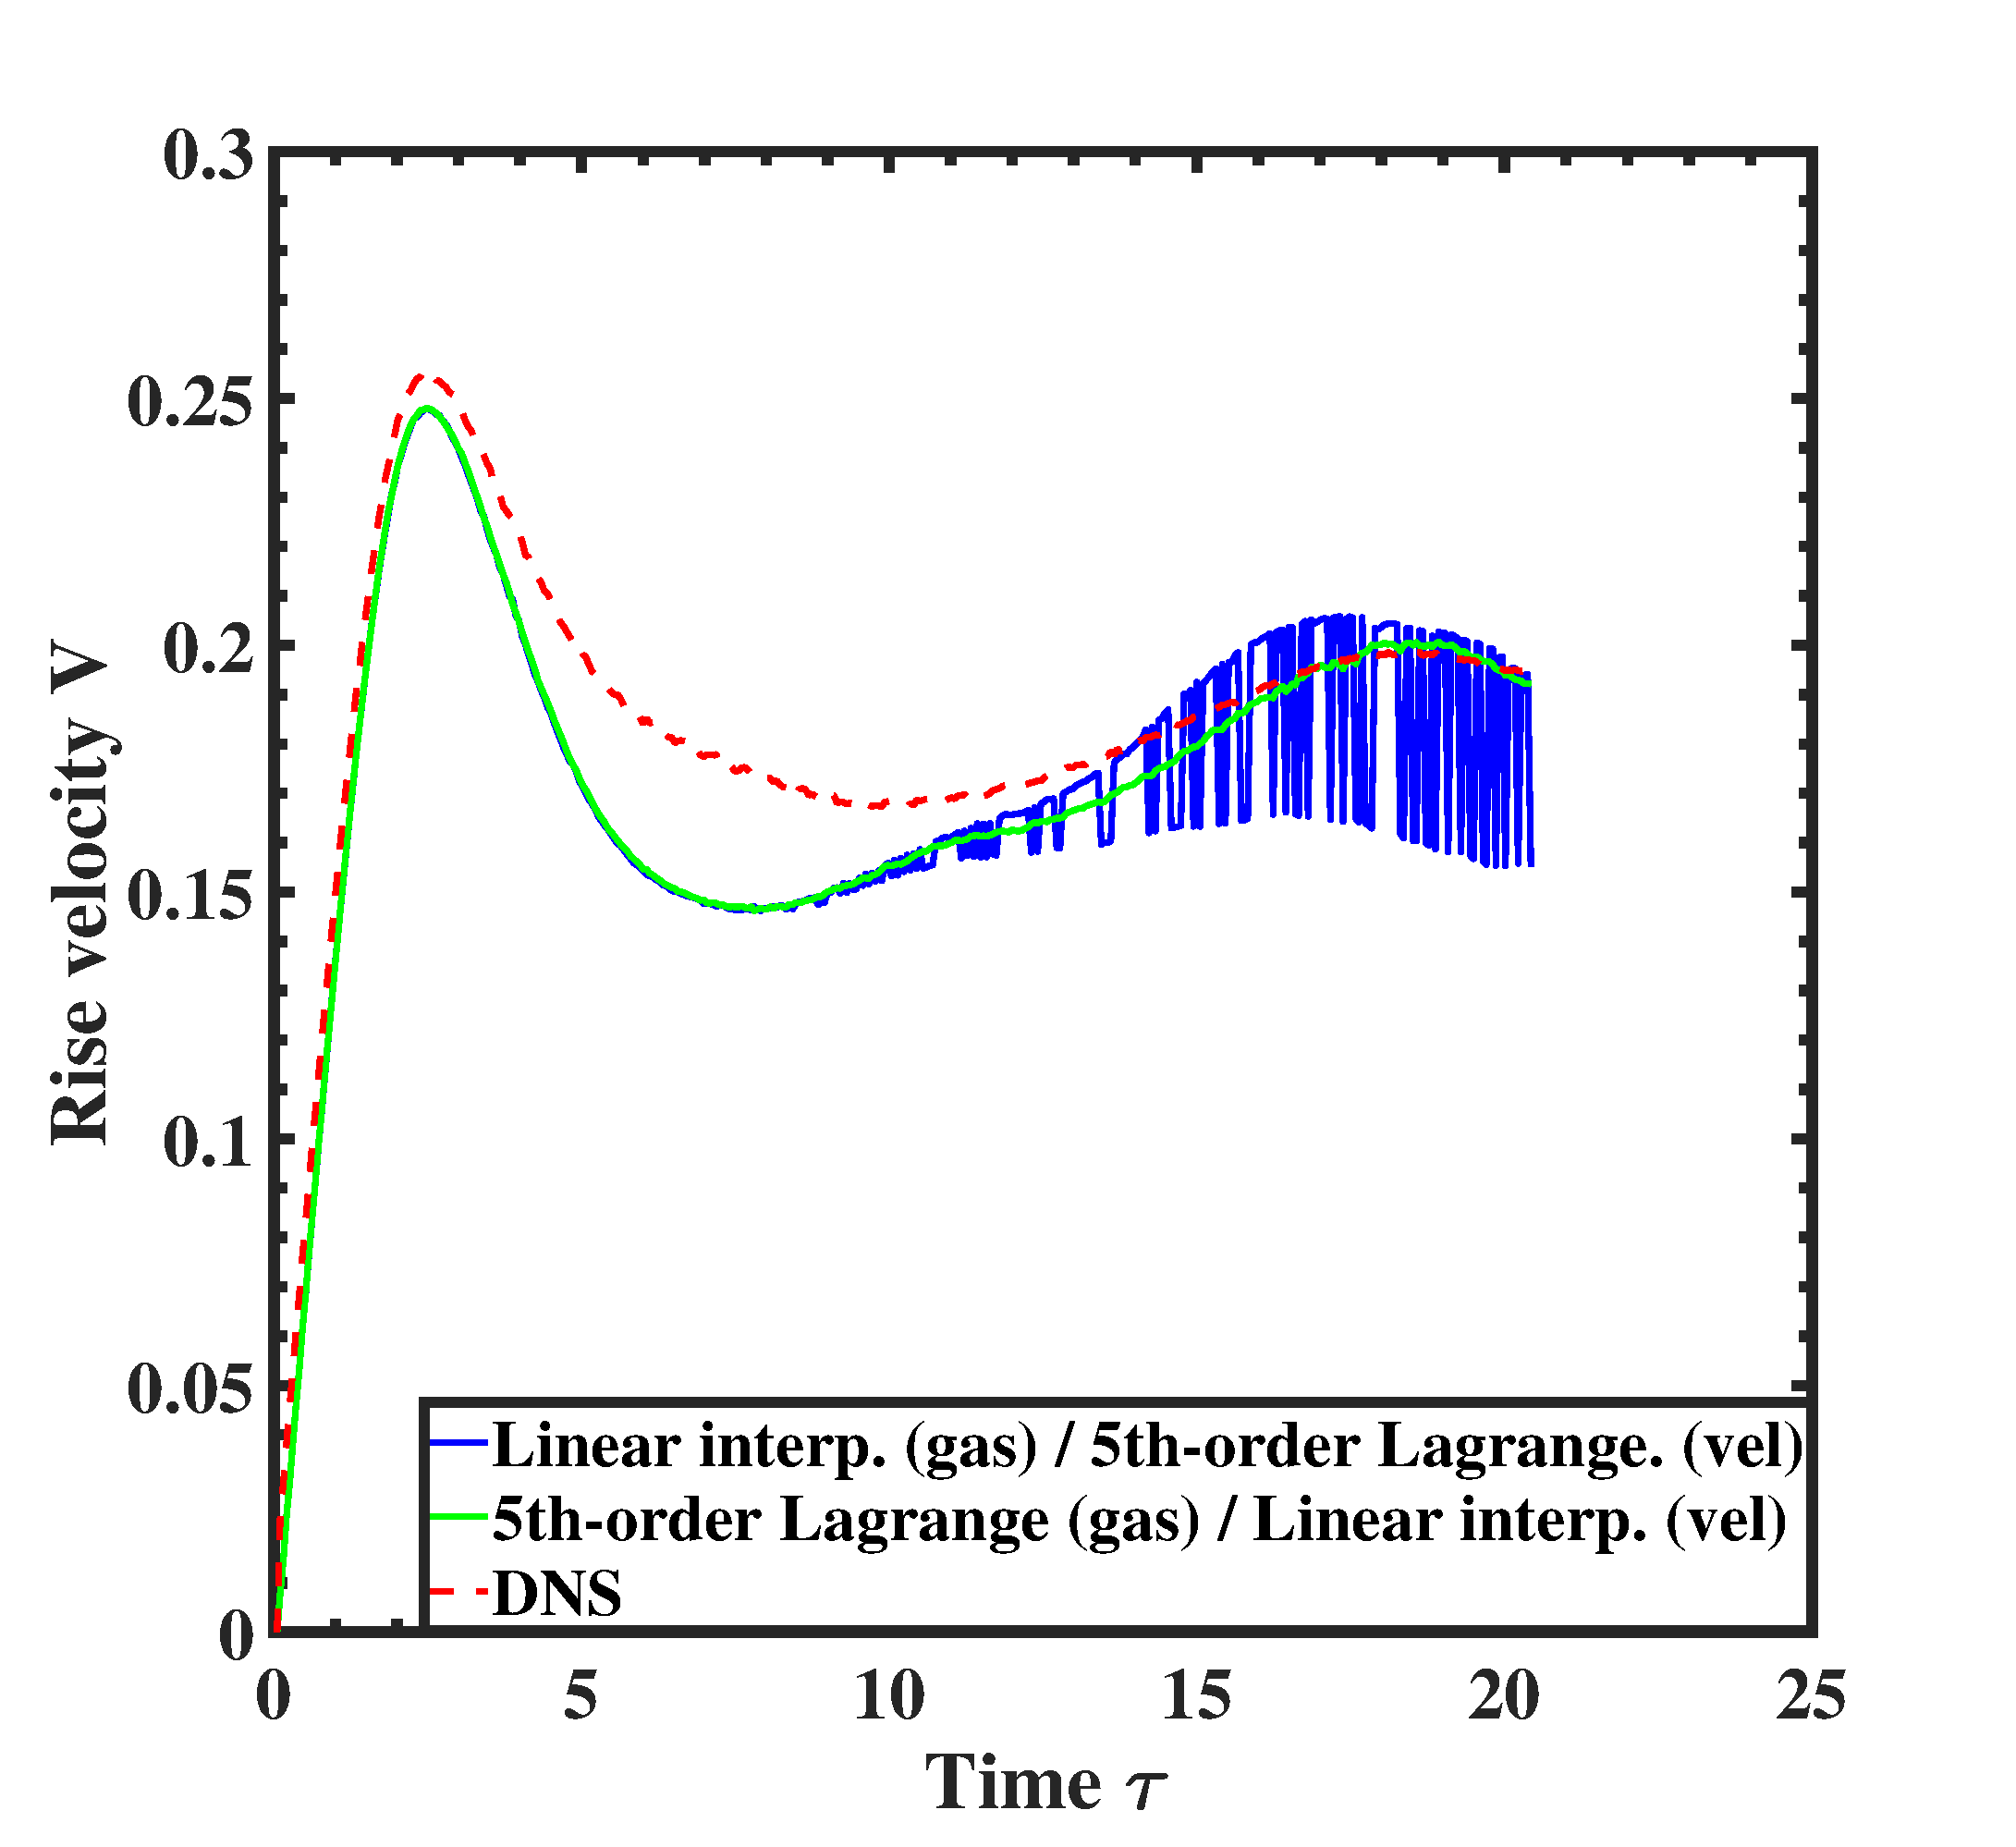
\includegraphics[scale=0.25,trim={00cm 00cm 0cm 0cm},clip]{Figure_A.1.eps}
		\caption{Sensitivity analysis of rise velocity to interpolation schemes for the bubble case C$_3$ using linear and 5th-order Lagrange functions.}
		\label{Fig.8}
	\end{figure}
	
	
	\section{Input and output observation values of data-driven methods and rank selection}
	\label{Append_B}
	
	\renewcommand{\theequation}{B.\arabic{equation}}
	\setcounter{equation}{0}
	
	\hl{The input and output data matrices for different frames of reference with their corresponding observation values are schematically shown in Fig.\ref{Fig9}. Rise velocity, the shape of the bubble and its centroid are the main characteristics studied in the present work. Thus, the upward component of the velocity and the gas volume fraction fields are considered. In the Lagrangian and \hl{moving-Eulerian} frames of reference, the set of coordinates of Lagrangian tracers and \hl{moving-Eulerian} grids should also be obtained during the rise process. Therefore, in these two frameworks, the coordinate matrix of the data points is also decomposed and later reconstructed. Obviously, the coordinates of the fixed Eulerian grid do not change and thus require no reconstruction. For the selected frame, the input data matrices of velocity ($V$), gas volume fraction ($G$), and coordinates ($P$) in stacked form are separately decomposed, and later a truncated representation using $r$ modes is reconstructed as $V'$, $G'$, and $P'$. In this way, both the shape and the velocity field are represented in the selected frame at their corresponding coordinate. The size of the input matrix varies in the number of rows depending on the number of data points and the number of components for each observation value. For example, the input matrix $G$ in the Eulerian frame for bubble C$_3$, with $m=400$ snapshots and a grid size of $n_r=250$ and $n_z=750$, is of size $(250 \times 750) \times 400$. For the same case in the Lagrangian frame, the $P$ matrix has the same number of columns with $n_s= (2\times250 \times 750)$ rows because it contains both components of the coordinates. It should be noted that, due to the scattered output of Lagrangian tracking, an interpolation of the scattered data points onto a uniform grid is required to represent the bubble interface, whereas the Eulerian and \hl{moving-Eulerian} frames are already defined on their original uniform grids.}
	
	\begin{figure}[h]
		\centering
		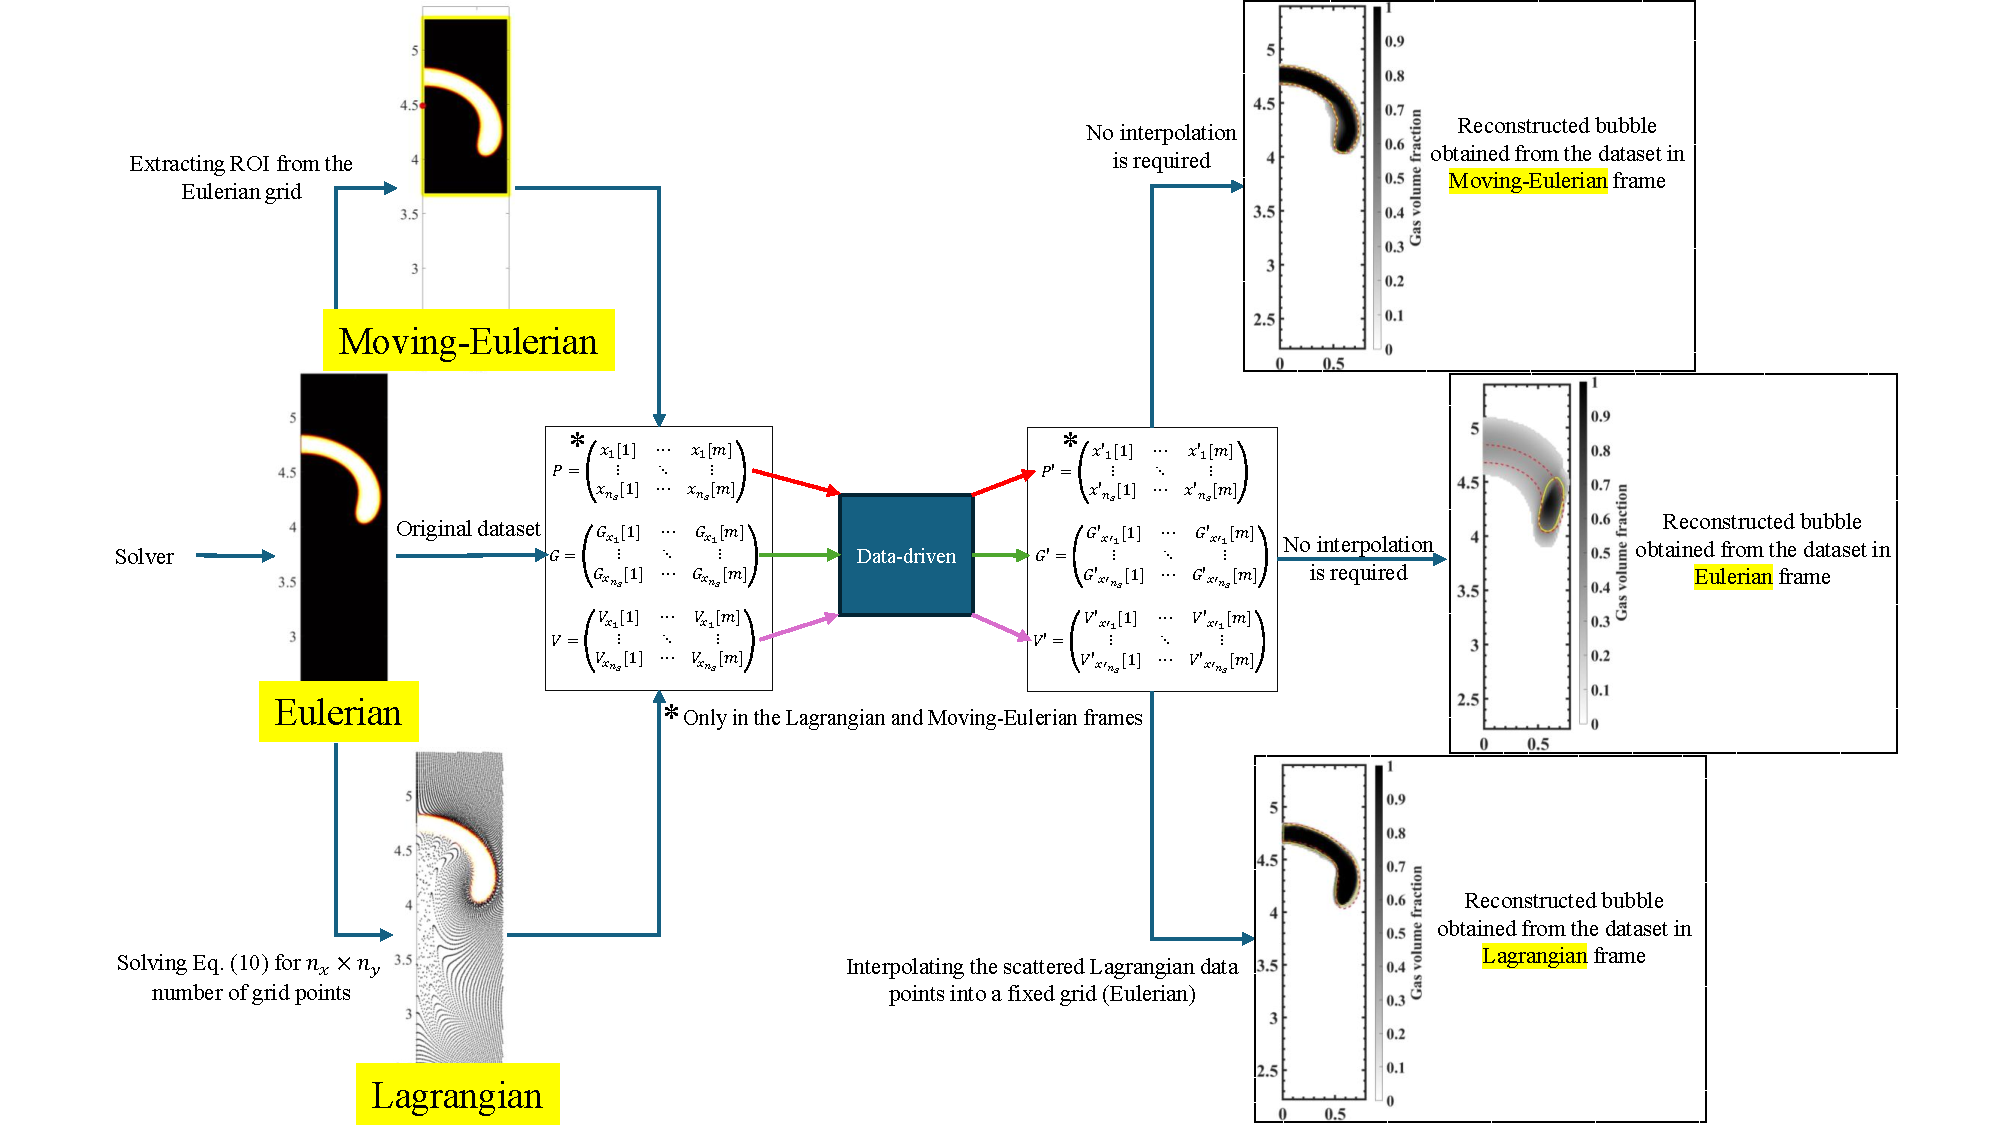
\includegraphics[scale=0.54,trim={1.8cm 00cm 1cm 0cm},clip]{Figure_B.1.pdf}
		\caption{Schematic of input and output data matrices of data-driven methods.}
		\label{Fig9}
	\end{figure}
	
	The truncated representation of $\mathcal{D}_r$ utilizes the first $r$ number of modes, selected based on the threshold value for cumulative variability, also known as cumulative energy, given by
	
	
	\begin{equation}
		\begin{aligned}
			C_e(r) = \frac{\sum\limits_{j=1}^r {\lambda_j}}{\sum\limits_{j=1}^m{\lambda_j}} \times 100 > 99
		\end{aligned} \label{eqB1}
	\end{equation}
	
	It is a common practice to select the truncation rank $r$ such that it captures $95$--$99$\% of the total variance in the system while discarding the remaining modes. In this expression, $\lambda_j$ is the eigenvalue of the $j^{th}$ mode obtained in Eq.~\ref{eq 4}. As shown in Fig.\ref{Fig10}, the most complex case with large deformation and zigzag rise trajectory is the bubble case C$_5$, whose cumulative energy is 99.2\% using 10 modes in the \hl{moving-Eulerian} framework for both velocity and gas volume fraction. As illustrated, using the same number of modes satisfies the aforementioned energy criterion for bubble case C$_3$ in the \hl{moving-Eulerian} and Lagrangian frameworks. \hl{It is worth mentioning that for the coordinate matrices of Lagrangian particles and the \hl{moving-Eulerian} frame, the cumulative energy criterion reaches 99\% with only 1 mode, reflecting the inherently low-rank/compact structure of particle positions compared to the more dispersive velocity and gas volume fraction fields. Thus, a single-mode reconstruction is considered for the coordinates of the Lagrangian and moving-Eulerian data points unless otherwise specified.}
	
	\begin{figure}[!t]
		\centering
		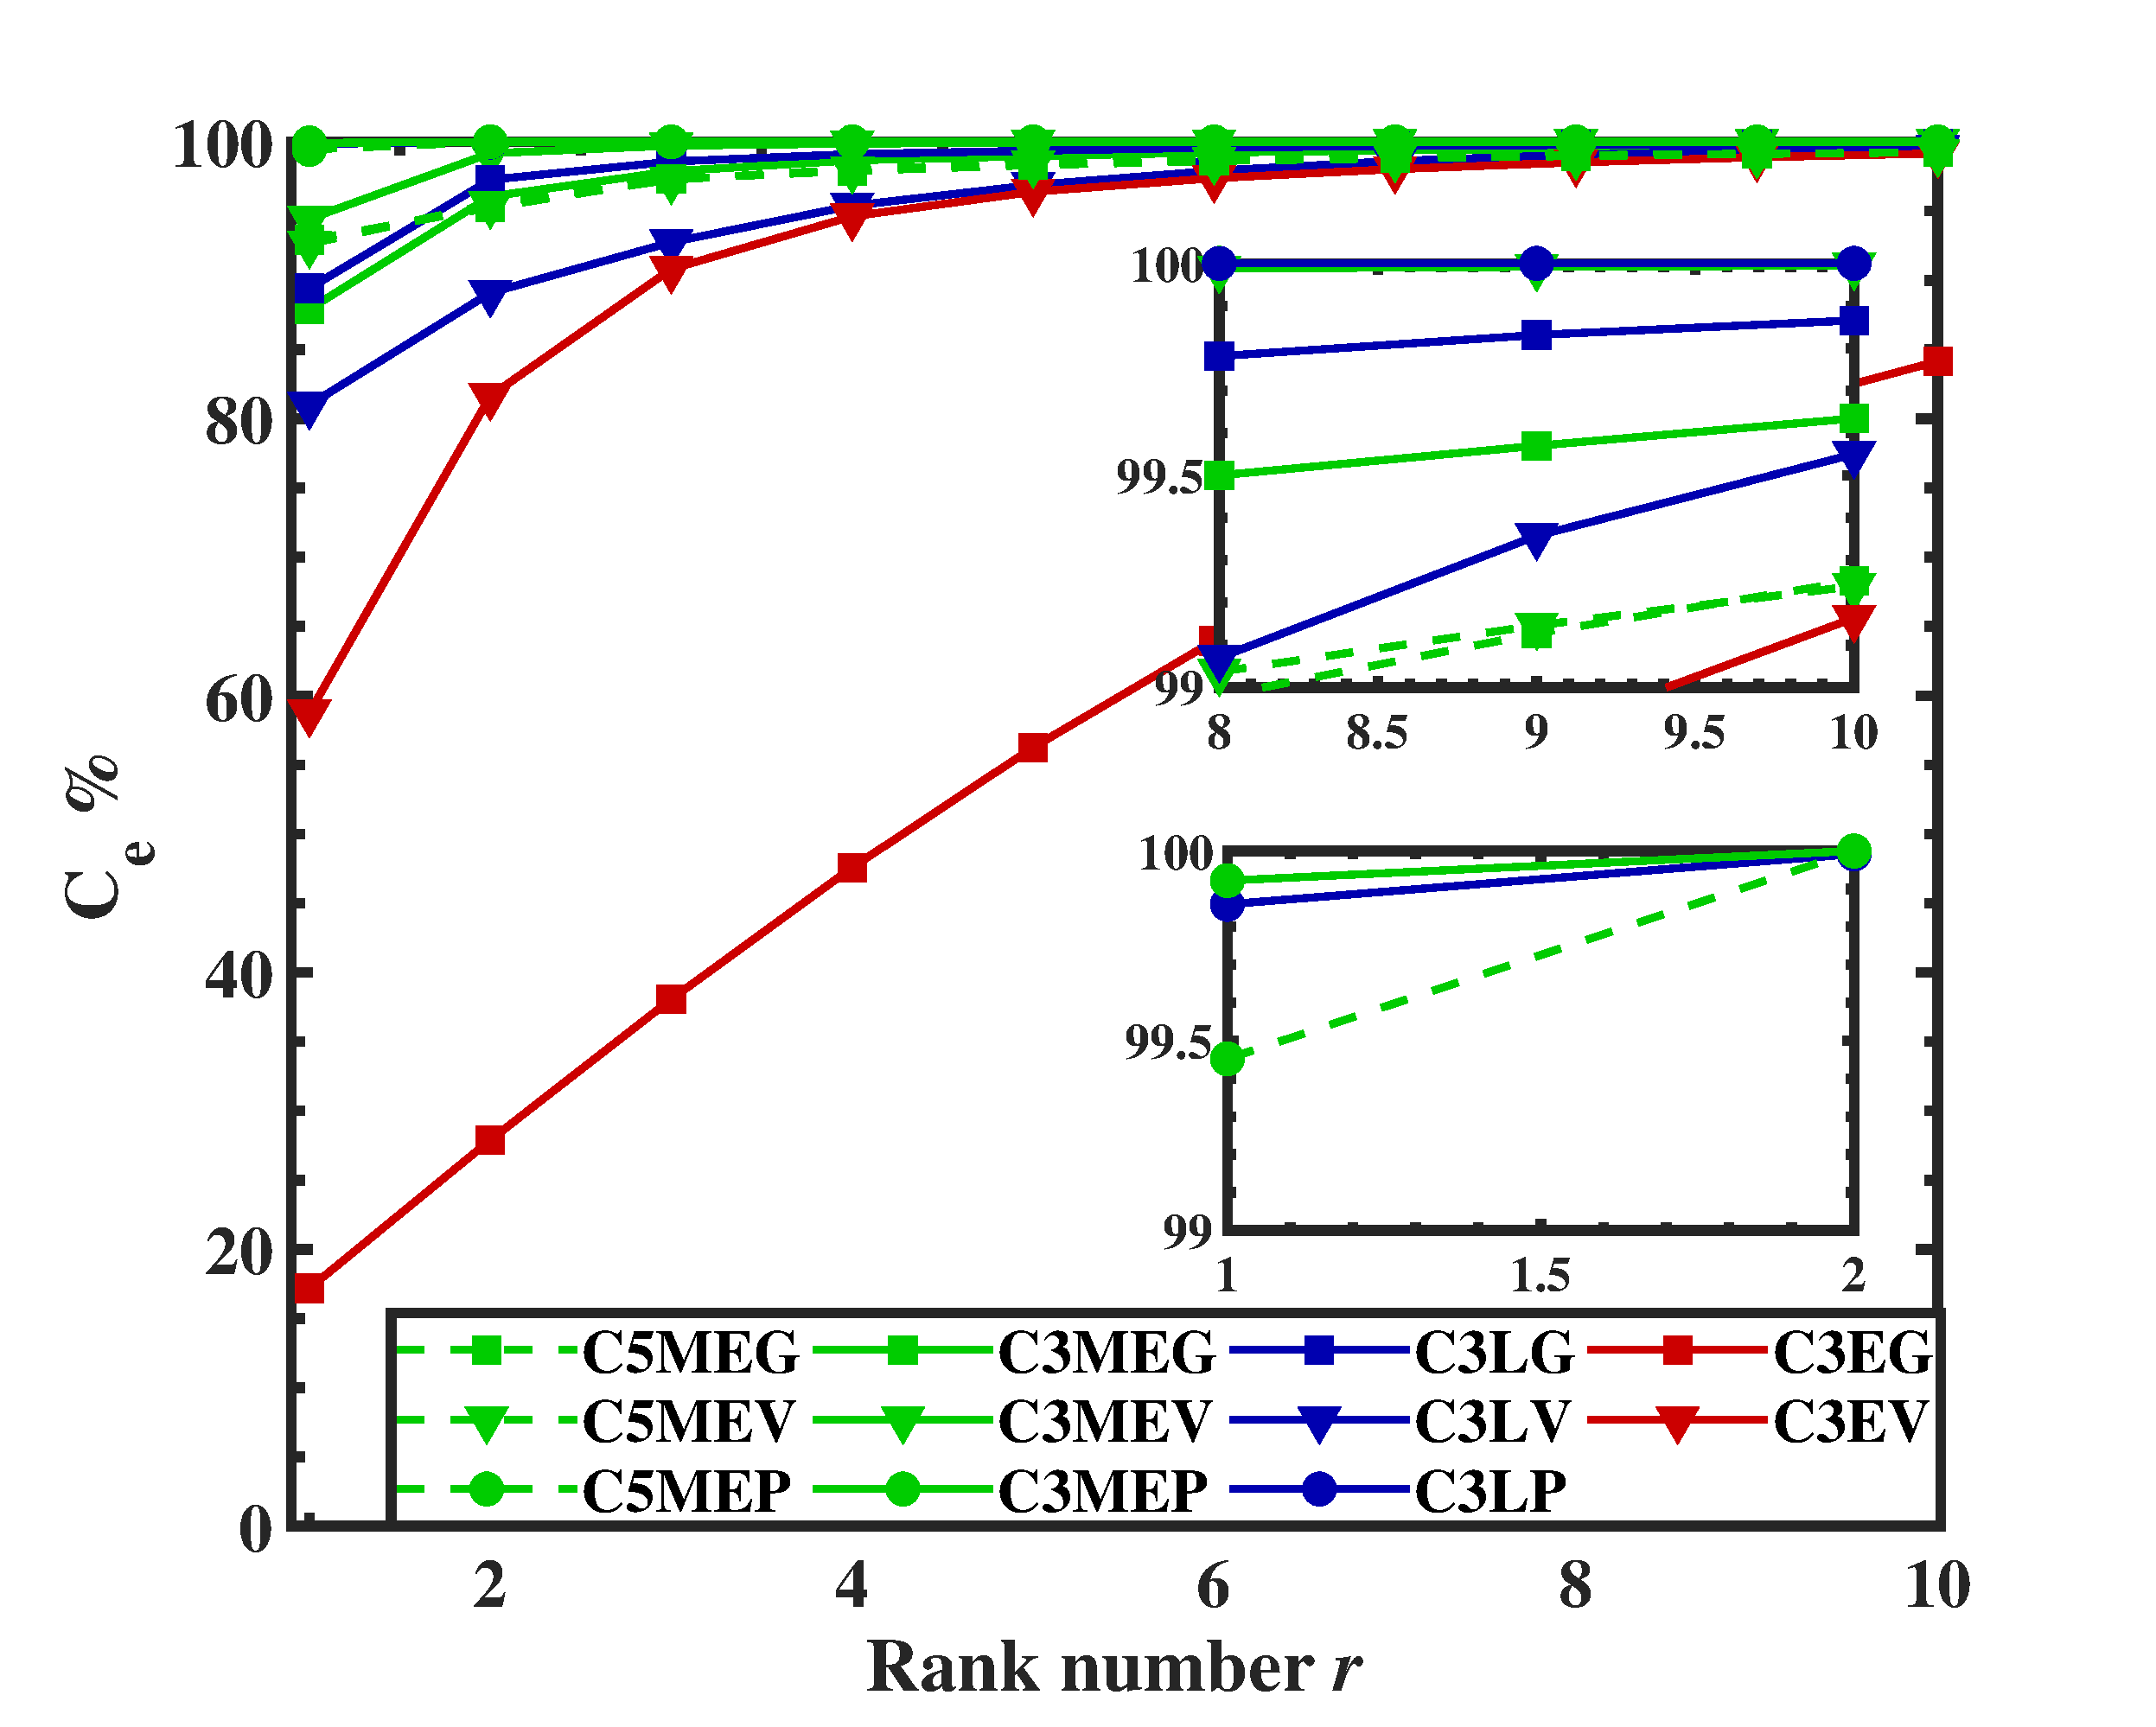
\includegraphics[scale=0.25,trim={00cm 00cm 0cm 0cm},clip]{Figure_B.2.eps}
		\caption{Rank selection based on the cumulative energy profile for bubble cases C$_5$ (dashed-line) and C$_3$ (solid line) within Eulerian (red), Lagrangian (blue), and \hl{moving-Eulerian} (green) frameworks. Square, circle and triangle markers denote gas volume (G), upward velocity component (V) and coordinates datasets (P).}
		\label{Fig10}
	\end{figure}
	

\nolinenumbers % <-- Stop line numbering

\clearpage

	%% Loading bibliography style file
	%\bibliographystyle{model1-num-names}
	%\bibliographystyle{cas-model2-names}
	\bibliographystyle{elsarticle-num-names}
	% Loading bibliography database
	\bibliography{library}
	
	
\end{document}

